
\documentclass[a4paper,12pt, oneside]{book}

%\usepackage{fullpage}
\usepackage[italian]{babel}
\usepackage[utf8]{inputenc}
\usepackage{amssymb}
\usepackage{amsthm}
\usepackage{graphics}
\usepackage{amsfonts}
\usepackage{amsmath}
\usepackage{amstext}
\usepackage{engrec}
\usepackage{rotating}
\usepackage[safe,extra]{tipa}
\usepackage{showkeys}
\usepackage{multirow}
\usepackage{hyperref}
\usepackage{microtype}
\usepackage{enumerate}
\usepackage{braket}
\usepackage{marginnote}
\usepackage{pgfplots}
\usepackage{cancel}
\usepackage{polynom}
\usepackage{booktabs}
\usepackage{enumitem}
\usepackage{framed}
\usepackage{pdfpages}
\usepackage{pgfplots}
\usepackage{fancyhdr}

\usepackage{varwidth,pst-tree,realscripts}
\usepackage{bidi}
\usetikzlibrary{automata,positioning}
\psset{showbbox=false,treemode=D,linewidth=0.3pt,treesep=2ex,levelsep=0.5cm}
\newcommand{\LFTw}[2]{%
\Tr[ref=#1]{\psframebox[linestyle=none,framesep=4pt]{%
\begin{varwidth}{15ex}\center #2\end{varwidth}}}}
\newcommand{\LFTr}[2]{\Tr[ref=#1]{\psframebox[linestyle=none,framesep=4pt]{#2}}}

\def\pstreehooki{\psset{thislevelsep=*0pt}}
\def\pstreehookiii{\psset{thislevelsep=*0pt}}
\def\pstreehookv{\psset{thislevelsep=*0pt}}

\pagestyle{fancy}
\fancyhead[LE,RO]{\slshape \rightmark}
\fancyhead[LO,RE]{\slshape \leftmark}
\fancyfoot[C]{\thepage}



\title{Linguaggi e Computabilità}
\author{UniShare\\\\Davide Cozzi\\\href{https://t.me/dlcgold}{@dlcgold}\\\\Gabriele De Rosa\\\href{https://t.me/derogab}{@derogab} \\\\Federica Di Lauro\\\href{https://t.me/f_dila}{@f\textunderscore dila}}
\date{}

\pgfplotsset{compat=1.13}
\begin{document}
\maketitle

\definecolor{shadecolor}{gray}{0.80}

\newtheorem{teorema}{Teorema}
\newtheorem{definizione}{Definizione}
\newtheorem{esempio}{Esempio}
\newtheorem{corollario}{Corollario}
\newtheorem{lemma}{Lemma}
\newtheorem{osservazione}{Osservazione}
\newtheorem{nota}{Nota}
\tableofcontents
\renewcommand{\chaptermark}[1]{%
\markboth{\chaptername
\ \thechapter.\ #1}{}}
\renewcommand{\sectionmark}[1]{\markright{\thesection.\ #1}}

\chapter{Introduzione}
\textbf{Questi appunti sono presi a lezione. Per quanto sia stata fatta una revisione è altamente probabile (praticamente certo) che possano contenere errori, sia di stampa che di vero e proprio contenuto. Per eventuali proposte di correzione effettuare una pull request. Link: } \url{https://github.com/dlcgold/Appunti}.\\
\textbf{Grazie mille e buono studio!}
\section{Definizioni}
\begin{itemize}
\item un \textbf{linguaggio }è un insieme di stringhe che può essere generato mediante un dato meccanismo con delle date caratteristiche; un linguaggio può essere riconosciuto, ovvero dando in input una stringa un meccanismo può dirmi se appartiene o meno ad un linguaggio. I meccanismi che generano linguaggi si chiamano \textit{grammatiche}, quelli che li riconoscono \textit{automi}. I linguaggi formali fanno parte dell'informatica teorica \textit{(TCS)}
\item si definisce \textbf{alfabeto} come un insieme finito e non vuoto di simbolo (come per esempio il nostro alfabeto o le cifre da 0 a 9). Solitamente si indica con $\Sigma$ o $\Gamma$
\item si definisce \textbf{stringa} come una sequenza finita di simboli (come per esempio una parola o una sequenza numerica). La stringa vuota è una sequenza di 0 simboli, e si indica con $\varepsilon$ o $\lambda$
\item si definisce \textbf{lunghezza di una stringa} il numero di simboli che la compone (ovviamente contando ogni molteplicità). Se si ha $w\in \Sigma^*$ è una stringa $w$ con elementi da $\Sigma^*$ (insieme di tutte le stringhe di tutte le lunghezze possibili fatte da $\Sigma$), allora $|w|$ è la lunghezza di $w$, inoltre $|\varepsilon|=0$.
\item si definisce \textbf{potenza di un alfabeto} $\Sigma^k$ come l'insieme di tutte le sequenze (espressi come stringhe e non simboli) di lunghezza $k\in\mathbb{N},\, k>0$ ottenibili da quell'alfabeto (se $\Sigma^2$ si avranno tutte le sequenza di 2 elementi etc...). Se ho $k=1$ si ha $\Sigma^1\neq \Sigma$ in quanto ora ho stringhe e non simboli. Se ho $k=0$ ho $\Sigma^0=\varepsilon$. Dato $k$ ho $|\Sigma|$ che è la cardinalità dell'insieme $\Sigma$ (e non la sua lunghezza come nel caso delle stringhe); sia $w\in\Sigma^k=a_1,a_2,...,a_k,\,a_i\in\Sigma$ e $|\Sigma|=q$ ora: $$|\Sigma^k|=q^k$$
\item si definisce $\Sigma^*$ come\textbf{ chiusura di Kleene} che è l'unione infinita di $\Sigma^k$ ovvero $$\Sigma*=\Sigma^0\cup \Sigma^1\cup...\cup \Sigma^k$$
\item si ha che $\Sigma^+$ è l'unione per $k\geq 1$ di $\Sigma^k$ ovvero:
$$\Sigma+=\Sigma^1\cup \Sigma^2\cup...\cup \Sigma^k= \Sigma^*-\Sigma^0$$
per esempio, per l'insieme $\{0,1\}$ si ha:
$$\Sigma^*=\{\varepsilon,0,1,00,01,10,100,000,...\}$$
\item quindi un \textbf{linguaggio} \textit{L} è un insieme di stringhe e:
$$L\subseteq \Sigma^*$$ 
si hanno sottoinsiemi particolari, come l'insieme vuoto, che resta però un linguaggio, il \textbf{linguaggio vuoto} e $\emptyset\in\Sigma^k,\,|\emptyset|=0$ che è diverso dal linguaggio che contiene la stringa vuota $|\varepsilon|=1$ (che conta come una stringa). Inoltre $\Sigma^*\subseteq \Sigma^*$ che ha lunghezza infinita. Posso concatenare due stringhe con un punto: $a\cdot b\cdot c=abc$ e $a\cdot \varepsilon=a$. Ovviamente la stringa concatenata è lunga come la somma delle lunghezze delle stringhe che la compongono. Vediamo qualche esempio di linguaggio:
\begin{itemize}
\item il linguaggio di tutte le stringhe che consistono in $n$ 0 seguiti da $n$ 1:
$$\{\varepsilon,01,0011,000111,...\}$$
\item l'insieme delle stringhe con un uguale numero di 0 e di 1:
$$\{\varepsilon,01,10.0011,0101.1001,..\}$$
\item l'insieme dei numeri binari il cui valore è un numero primo:
$$\{\varepsilon,10 , 11, 101, 111,1011,...\}$$
\item $\Sigma^*$ è un linguaggio per ogni alfabeto $\Sigma$
\item $\emptyset$, il linguaggio vuoto, e $\{\varepsilon\}$ sono un linguaggio rispetto a qualunque alfabeto
\end{itemize}
\end{itemize}
Prendiamo un alfabeto $\Sigma=\{0, 1\}$ con la sua chiusura di Kleen $\Sigma=\{0, 1\}^*$. Quando si ha un input si può avere un problema di decisione, \textit{P}, che dia come output "si" o "no". Posso avere un problema di decisione (o \textit{membership}) su $w\in\Sigma=\{0, 1\}^*$, con \textit{w} stringa, che dia in output "si" o "no". Un linguaggio \textit{L} sarà:
$$L=\{w\in\{0, 1\}^*\,|\,\, P(w)=si$$
quindi si ha che:
$$\Sigma^*\backslash L=\{P(w)=no\}$$
Vediamo ora un esempio di \textit{Context Free Language (CFL)}, costruito a partire da una \textit{Context Free Grammar (CFG)}:
\begin{esempio}
Sia $\Sigma=\{0, 1\}$ e $L_{pal}="stringhe\,\, palindrome\,\, binarie"$.
Quindi, per esempio, $0110\in L,\,\, 11011\in L$ ma $10010\not\in L$. Si ha che $\varepsilon$, la stringa vuota, appartiene a $L$. Diamo una definizione ricorsiva:
\begin{itemize}
\item \textbf{base:} $\varepsilon,\, 0\,\ 1\in L_{pal}$
\item \textbf{passo:} se $w$ è palindroma allora $0w0$ è palindromo e $1w1$ è palindromo
\end{itemize}
una variabile generica $S$ può sottostare alle \textit{regole di produzione} di una certa grammatica. In questo caso si ha uno dei seguenti:
$$S\to\varepsilon,\, S\to 0,\, S\to 1,\, S\to 0S0,\, S\to 1S1$$
\end{esempio}
Si ha che una grammatica $G$ è una quadrupla $G=(V,\,T,\,P,\,S)$ con:
\begin{itemize}
\item $V$ simboli variabili
\item $T$ simboli terminali, ovvero i simboli con cui si scrivono le stringhe alla fine
\item $P$ regole di produzione
\item $S$ variabile di partenza \textit{start}
\end{itemize}
riprendiamo l'esempio sopra:
\begin{esempio}
$$G_{pal}=(V=\{S\},\, T=\{0, 1\},\, P,\, S)$$
con:
$$P=\{S\to\varepsilon,\, S\to 0,\, S\to 1,\, S\to 0S0,\, S\to 1S1\}$$
Si può ora costruire un algoritmo per creare una stringa palindroma a partire dalla grammatica $G$:
$$\underbrace{S}_{\mbox{start}}\underbrace{\to}_{\mbox{applico una regola}} 1S1 \to 01S10\to \underbrace{01010}_{\mbox{sostituisco variabile}}$$

con $S,\, 1S1\,\, e\,\, 01S10$ che sono \textit{forme sentenziali}. Posso così ottenere tutte le possibili stringhe. Esiste anche una forma abbreviata:
$$S\to \varepsilon|o|1|0S0|1S1$$
Non si fanno sostituzioni in parallelo, prima una $S$ e poi un'altra
\end{esempio}
%aggiungi esempio parentesi
Si hanno 4 grammatiche formali, \textit{gerarchia di Chomsky}:
\begin{itemize}
\item \textbf{tipo 0:} non si hanno restrizioni sulle regole di produzione, $\alpha\to\beta$. Sono linguaggi ricorsivamente numerabili e sono rappresentati dalle \textit{macchine di Turing}, deterministiche o non deterministiche (la macchina di Turing è un automa)
\item \textbf{tipo 1:}  il lato destro della produzione ha lunghezza almeno uguale a quello sinistro. Sono grammatiche dipendenti dal contesto (\textit{contestuali}) e come automa hanno\textit{ la macchina di Turing che lavora in spazio lineare}:
$$\alpha_1A\alpha_2\to \alpha_1B\alpha_2$$
con $\alpha_1$ e $\alpha_2$ detti \textit{contesto} e $\alpha_1,\,\alpha_2,\, \beta\in (V\cup T)^*$
\item \textbf{tipo 2:} sono quelle libere dal contesto, context free. Come regola ha $A\to\beta$ con $A\in V$ e $\beta\in V\cup T)^*$ e come automa ha gli \textit{automi a pila non deterministici}
\item \textbf{tipo 3:} sono le grammatiche \textit{regolari}. Come regole ha $A\to\alpha B$ (o $A\to B\alpha$) e $A\to\alpha$  con $A,B\in V$ e $\alpha\in T$. Come automi ha gli \textit{automi a stato finito deterministici o non deterministici}
\end{itemize}
%aggiungi esercizio
\newpage
\begin{esempio}
Sia $G=(V,T,O,E)$, con $V=\{E,I\}$ e $T=\{a,b,0,1,(,),+,*\}$ 
quindi ho le seguenti regole, è di tipo 3:
\begin{enumerate}
\item $E\to I$
\item $E\to E+E$
\item $E\to E*E$
\item $E\to (E)$
\item $I\to a$
\item $I\to b$
\item $I\to Ia$
\item $I\to Ib$
\item $I\to I0$
\item $I\to I1$
\end{enumerate}
voglio ottenere $a*(a+b00)$ 
sostituisco sempre a destra (right most derivation)
$$E\to E*E\to E*(E)\to E*(E+E)\to E*(E+I)\to E+(E+I0)$$
$$\to R+(I+b00)\to E*(a+b00)\to I*(a+b00)\to a*(a+b00)$$

usiamo ora \textit{l'inferenza ricorsiva}:
\begin{center}
\begin{tabular}{|c|c|c|c|c|}
\hline
passo & stringa ricorsiva & var & prod & passo stringa impiegata\\
1 & a & I & 5 & $\backslash$ \\
\hline
2 & b & I & 6 & $\backslash$ \\ 
\hline
3 & b0 & I & 9 & 2\\
\hline
4 & b00 & I & 9 & 3\\
\hline
5 & a & E & 1 & 1 \\
\hline
6 & b00 & E & 1 & 4\\
\hline
7 & a+b00 & E & 2 & 5,6\\
\hline
8 & (a+b00) & E & 4 & 7\\
\hline
9 &a*(a+b00) & E & 3 & 5, 8\\
\hline
\end{tabular}
\end{center}
\end{esempio}
definisco formalmente la derivazione $\to$:
\begin{definizione}
Prendo una grammatica $G=(V,T,P,S)$, grammatica CFG. Se $\alpha A \beta$ è una stringa tale che $\alpha,\beta\in (V\cup T)^*$, appartiene sia a variabili che terminali. Sia $A\in V$ e sia $a\to \gamma$ una produzione di $G$. Allora 
scriviamo:
$$\alpha A \beta \to \alpha\gamma\beta$$
con $\gamma\in (V\cup T)^*$.\\
Le sostituzioni si fanno indipendentemente da $\alpha$ e $\beta$.
Questa è quindi la definizione di derivazione.
\end{definizione}
\begin{definizione}
Definisco il simbolo $\to _*$, ovvero il simbolo di \textit{derivazioni in 0 o più passi}. Può essere definito in modo ricorsivo. Per induzione sul numero di passi.
\begin{itemize}
\item la base dice che  $\forall \alpha\in (V\cup T)^*,\, \alpha\to * \,\alpha$
\item il passo è: se $\alpha\to_G * \,\beta $ e $ \beta \to_G * \,\gamma$ allora $\alpha\to * \,\gamma$
\end{itemize}
Si può anche dire che $\alpha\to_G *\, \beta$ sse esiste una sequenza di stringhe $\gamma_1,...,\gamma_n$ con $n\geq 1$ tale che $\alpha=\gamma_1$, $\beta=\gamma_n$ e $\forall i,\, 1<i<n-1$ si ha che $\gamma_1\to \gamma_{i+1}$
la derivazione in 0 o più passi è la chiusura transitiva della derivazione
\end{definizione}
\begin{definizione}
avendo ora definito questi simboli possiamo definire una forma sentenziale. Infatti è una stringa $\alpha$ tale che:
$$\forall \alpha\in (V\cup T)^* \mbox{ tale che }S\to_G *\, \alpha$$
\end{definizione}
\begin{definizione}
data $G=(V,T,P,S)$ si ha che $L(G)=\{w\in T^* |\, S\to_G *\, w\}$ ovvero composto da stringhe terminali che sono derivabili o 0 o più passi.
\end{definizione}
\begin{esempio}
formare una grammatica CFG per il linguaggio:
$$L=\{0^n 1^n| n\geq 1\}=\{01, 0011, 000111,...\}$$
con $x^n$ intendo una concatenazione di $n$ volte $x$ (che nel nostro caso sono 0 e 1).\\
posso scrivere:
$$0^n 1^n =00^{n-1} 1^{n-1}1$$
il nostro caso base sarà la stringa $01$, Poi si ha:
$G=(V,T,P,S)$, $T=\{0,1\}$, $V=\{S\}$, il caso base $S\to 01$  e $S\to 0S1$
il caso passo è quindi: se $w= 0^{n-1}1^{n-1}\in L$ allora $0w1\in L$.\\
Ora voglio dimostare che $000111\in L$, ovvero $S\to*\, 000111$:\\
$$S\to\, 0S1 \to 00S11\to 000S111$$
\end{esempio}
\begin{teorema}
data la grammatica $G=\{V,T,P,S)$ CFG e $\alpha\in (V\cup T)^*$. Si ha che vale $S\to*\, \alpha$ sse $S\to_{lm}*\, \alpha$ sse $S\to_{rm}*\, \alpha$. Con $\to_{lm}*$ simbolo di \textit{left most derivation }e $\to_{rm}*$ simbolo di \textit{right most derivation}
\end{teorema}
\begin{esempio}
formare una grammatica CFG per il linguaggio:
$$L=\{0^n 1^n| n\geq 0\}=\{\varepsilon, 01, 0011, 000111,...\}$$
stavolta abbiamo anche la stringa vuota. Il caso base stavolta è $S\to\varepsilon| \, 0S1$ 
\end{esempio}
\begin{esempio}
Fornisco una CFG per $L=\{a^n|n\geq 1\}=\{a, aa, aaa,...\}$.
La base è $a$ \\il passo è che se $a^{n-1}\in L$ allora $a^{n-1}a\in L$ ( o che $aa^{n-1}\in L$).\\
Si ha la grammatica $G=\{V,T,P,S)$, $V=\{S\}$, $T=\{a\}$ e si hanno $S\to a|\,Sa$ (o  $S\to a|\,aS$). Dimostro che $a^3\in L$.
$$S\to Sa \to Saa\to aaa$$
oppure 
$$S\to aS\to aaS\to aaa$$
\end{esempio}
\begin{esempio}
trovo una CFG per $L=\{(ab)^n|n\geq 1\}=\{ab, abab, ababab,...\}$\\
La base è $ab$ \\il passo è che se $(ab)^{n-1}\in L$ allora $(ab)^{n-1}ab\in L$.\\
Si ha la grammatica $G=\{V,T,P,S)$, $V=\{S\}$, $T=\{a,b\}$ (anche se in realtà $T=\{ab\}$) e si hanno $S\to ab|\,Aab$. Poi dimostro come l'esempio sopra
\end{esempio}
\begin{esempio}
trovo una CFG per $L=\{a^n c b^n|n\geq 1\}=acb,aacbb,aaacbbb,...\}$\\
Il caso base è $acb$ il passo è che se $a^{n-1}cb^{n-1}\in L$ allora $a^{n-1}cb^{n-1}acb\in L$ 
Si ha la grammatica $G=\{V,T,P,S)$, $V=\{S\}$, $T=\{a,b,c\}$ e si hanno $S\to aSb|acb$.\\
dimostro che $aaaacbbbbb\in L$:
$$S\to aSb\to aaSbb\to aaaaSbbb\to aaaacbbbb$$

provo a usare anche una grammatica regolare, con le regole $S\to aS|c$, $c\to cB$ e $B\to bB|b$;
$$S\to aS\to aaS\to aaC\to aacB\to aacb...$$
non si può dimostrare in quanto non si può imporre una regola adatta
\end{esempio}
\begin{esempio}
$L=\{a^n c b^{n-1}|n\geq 2\}$, con $a^n c b^{n-1}=a^{n-1}acb^{n-1}$. $S\to aSb|aacb$. Quindi:
$$S\to aSb\to aaaccbb\in L$$
\end{esempio}
\begin{esempio}
cerco CFG per $L=\{a^n c^k b^n|\,n,\,k>0\}$. $a$ e $b$ devono essere uguali, uso quindi una grammatica context free, mentre $c$ genera un linguaggio regolare.\\
Si ha la grammatica $G=\{V,T,P,S)$, $V=\{S,C\}$, $T=\{a,b,c\}$ e si hanno $S\to aSb|aCb$ e $C\to cC|c$. dimostro che $aaaccbbb\in L, n=3,\, k=2$:
$$S\to aSb \to aaSbb\to aaaCbbb\to aaacCbbb\to aaaccbbb$$
\end{esempio}
\begin{esempio}
scrivere CFG per $L=\{a^nb^nc^kb^k|\, n,\,k\geq 0\}
$
$$=\{w\in\{a,b,c,d\}^*|\,a^nb^nc^kb^k|\, n,\,k\geq 0\}$$
quindi L concatena due linguaggi $L1$ e $L2$, $X=\{a^nb^n\}$ e $Y=\{c^kd^k\}$: 
$$X\to aXb | \varepsilon$$
$$Y\to cYd | \varepsilon$$
$$S\to XY$$
voglio derivare $abcd$:
$$S\to XY \to XcYd\to aXbcYd\to aXbc\varepsilon d\to a\varepsilon bc\varepsilon d\to abcd$$
voglio derivare $cd$
$$S\to XY\to Y\to cYd\to cd$$
\end{esempio}
Quindi se ho $w\in L1, L2$, ovvero appartenente ad una concatenazione di linguaggi prima uso le regole di un linguaggio, poi dell'altro e infine ottengo il risultato finale.\\
\begin{esempio}
scrivere CFG per $L=\{a^nb^kc^kd^n|\, n>0,\, k\geq 0\}
$.
$$S\to aSd|\, aXd$$
$$X\to bXc| \varepsilon$$
derivo $aabcdd$:
$$S\to aSd\to aaXdd\to aabXcdd\to aabcdd$$
\end{esempio}
\begin{esempio}
scrivere CFG per $L=\{a^ncb^nc^mad^m|\, n>0,\, m\geq 1\}
$.
$$S\to XY$$
$$X\to aXb|c$$
$$Y\to cUd| cad$$
$$S\to XY\to cY\to ccad$$
\end{esempio}
\begin{esempio}
scrivere CFG per $L=\{a^{n+m}xc^nyd^m|\, n,\, m\geq 0\}
$. $a^{n+m}=a^na^m \mbox{ o } a^ma^n$. Si hanno 2 casi:
\begin{enumerate}
\item $L=\{a^na^m xc^nyd^m|\, n,\, m\geq 0\}
$
\item $L=\{a^ma^n xc^nyd^m|\, n,\, m\geq 0\}
$
\end{enumerate}
ma solo  $L=\{a^ma^n xc^nyd^m|\, n,\, m\geq 0\}
$ può generare una CFG (dove non si possono fare incroci, solo concatenazioni e inclusioni/innesti). 
$$S\to aSd| Y$$
$$Y\to Xy$$
$$X\to aXc|x$$ 
si può fare in 2:
$$S\to aSd| Xy$$
$$X\to aXc|x$$ 
derivo con $m=n=1$, $aaxcyd$:
$$S\to aSd\to aXyd\to aaXcyd\to aaxcyd$$
\end{esempio}
\begin{esempio}
scrivere CFG per $L=\{a^nb^m|\, n\geq m \geq 0\}
$.$$L=\{\varepsilon, a, ab, aa, aab, aabb, aaa, aaab, aaabb, aaabbb,...\}$$
Se $n\geq m$ allora $\exists k\geq 0 \to n=m+k$. Quindi:
$$l=\{a^{m+k}b^m|m,k\geq0\}$$ si può scrivere in 2 modi:
\begin{enumerate}
\item $l=\{a^ma^kb^m|m,k\geq0\}$ quindi con innesto
\item $l=\{a^ka^mb^m|m,k\geq0\}$quindi con concatenazione
\end{enumerate}
entrambi possibili per una CFG:
\begin{enumerate}
\item 
$$S\to XY$$
$$X\to aX|\varepsilon \mbox{ si può anche scrivere } X\to Xa|\varepsilon$$
$$Y\to aYb|\varepsilon$$ 
oppure 
$$S\to aS|X$$
$$X\to aXb| \varepsilon$$
\item 
$$S\to aSb|\varepsilon$$
$$X\to aX|\varepsilon$$
\end{enumerate}
\end{esempio}
\begin{esempio}
scrivere CFG per $L=\{a^nb^{m+n}c^h|\, m>h\geq0,\, n\geq0\}
$.\\
Se $n>h$ allora $\exists k \to n= h+k$, quindi:
$$L=\{a^nb^{m+h+k}c^h|\, m>h\geq0,\, n\geq0\}$$. ovvero:
$$L=\{a^nb^nb^kb^hc^h|\, m\geq 0, k>0, h\geq 0\}$$
si ha:
$$S\to XYZ$$
$$X\to aXb|\varepsilon$$
$$Y\to Yb|b$$
$$Z\to bZc|\varepsilon$$
si può anche fare:
$$S\to XY$$
$$X\to aXb|\varepsilon$$
$$Y\to bYc|Z$$
$$Z\to bZ|b$$
\end{esempio}
\begin{esempio}
scrivere CFG per $L=\{a^nb^mc^k|\, k>n+m,\, n,m\geq 0\}
$.\\
per $n=m=0,\, k=1$ avrò la stringa $c$.
se $k>n+m$ allora $\exists l>0\to k=n+m+l$ quindi:
$$L=\{a^nb^mc^{n+m+l}|\, l>0,\, n,m\geq 0\}
$$
$$=L=\{a^nb^mc^nc^mc^l|\, l>0,\, n,m\geq 0\}$$
sistemando:
$$=L=\{a^nb^mc^lc^mcnl|\, l>0,\, n,m\geq 0\}$$
quindi:
$$S\to aSc|X$$
$$X\to bXc|Y$$
$$Y\to cY|c$$
\end{esempio}
\newpage
\begin{esempio}
scrivere CFG per $L=\{a^nxc^{n+m}y^hz^kd^{m+h}|\, n,m,k,h\geq 0\}
$.\\
ovvero:
$$L=\{a^nxc^nc^my^hz^kd^hd^m|\, n,m,k,h\geq 0\}$$
quindi avrò:
$$S\to XY$$
$$X\to aXc|x$$
$$Y\to cYd|W$$
$$W\to yWd|X$$
$$Z\to zZ|\varepsilon$$
\end{esempio}
\begin{esempio}
vediamo un esempio di grammatica dipendente dal contesto:
$$L=\{a^nb^nc^n|\, n\geq 1\}$$
$G=\{V,T,P,S\}=\{(S,B,C,X)\}=\{(a,b,c),P,S\}$
ecco le regole di produzione (qui posso scambiare variabili a differenza delle context free):
\begin{enumerate}
\item $S\to aSBC$
\item $S\to aBC$
\item $CB\to XB$
\item $XB\to XC$
\item $XC\to BC$
\item $aB\to ab$
\item $bB\to bb$
\item $bC\to bc$
\item $cC\to cc$
\end{enumerate}
vediamo un esempio di derivazione:
per $n=1$ ho $abc$ ovvero:
$$S\to aBC\to abC\to abc$$
con $n=2$ ho $aabbcc$:
$S\to aSBC\to aaBCBC\to aaBXBC\to aaBXCC\to aaBBCC\to aabBCC\to aabbCC\to aabbcC\to aabbcc$\\
%vedere dimostrazione pag 14 soligo
\end{esempio}
\newpage
\begin{esempio}
vediamo un esempio di grammatica dipendente dal contesto:
$$L=\{a^nb^mc^nd^m|\, n,m\geq 1\}$$
Si ha:
$$G=(\{S,X,C,D,Z\},\{a,b,c,d\},P,S)$$
con le seguenti regole di produzione:
\begin{itemize}
\item $S\to aSc|\, aXc$
\item $X\to bXD|\, bD$
\item $DC\to CD$
\item $DC\to DZ$
\item $DZ\to CZ$
\item $XZ\to CD$
\item $bC\to bc$
\item $cC\to cc$
\item $cD\to cd$
\item $dD\to dd$
\end{itemize}
provo a derivare $aabbbccddd$ quindi con $n=2,\,m=3$:\\
$$S\to aSC\to aaXCC\to aabXDCC\to aabbXDDCC\to $$
$$aabbbDDDCC\to aabbbCCDDD\to aabbbccddd$$
\end{esempio}
\begin{esempio}
Sia $L=\{w\in\{a,b\}^*|\, \mbox{ w contiene lo stesso numero di a e b}\}$:
$$S\to aSbS|\,bSaS|\, \varepsilon$$
dimostro per induzione che è corretto:
\begin{itemize}
\item \textbf{caso base:} $|w|=0\to w=\varepsilon$
\item \textbf{caso passo:} si supponga che $G$ produca tutte le stringhe (di lunghezza $<$ di $n$) di $\{a,b\}^*$ con lo stesso numero di \textit{a} e \textit{b} e dimostro che produce anche quelle di lunghezza $n$, sia:
$$w\in \{a,b\}^* \mid\, |w|=n \mbox{ con\textit{ a} e \textit{b} in egual numero, }m(a)=m(b) \mbox{ con m() che indica il numero di caratteri}$$
quindi si ha che:
$$w=aw_1bw_2\mbox{ o } w=bw_1aw_2$$
sia.
$$k_1=m(a)\in w_1=m(b)\in w_1$$
$$k_2=m(a)\in w_2=m(b)\in w_2$$
allora:
$$k_1+k_2+1=m(a)\in w= m(b)\in W$$
sapendo che $|w_1|<n$ e $|w_2|<n$ allora $w_1$ e $w_2$ sono egnerati da G per ipotesi induttiva
\end{itemize}
\end{esempio}
\subsection{Alberi Sintatici}
\begin{definizione}
Data una grammatica CFG, $G=\{V,T,P,S\}$ un \textbf{albero sintattico} per $G$ soddisfa le seguenti condizioni:
\begin{itemize}
\item ogni nodo interno è etichettato con una variabile
\item ogni foglia è anch'essa etichettata con una variabile o col simbolo di terminale T o con la stringa vuota $\varepsilon$ (in questo caso la foglia è l'unico figlio del padre)
\item se un nodo interno è etichettato con A i suoi figli saranno etichettati con X1, ..., Xk e $A\to  X1, ..., Xk$ sarà una produzione di $G$. Se un Xi è $\varepsilon$ sarà l'unica figlio e $A\to \varepsilon$ sarà comunque una produzione di $G$
\end{itemize}
La concatenazione in ordine delle foglie viene detto \textbf{prodotto dell'albero}
\end{definizione}
\newpage
\begin{esempio}
Usiamo l'esempio delle stringhe palindrome:
$$P\to 0P0|\,1P1|\varepsilon$$
sia il seguente albero sintatico:
\begin{center}
\psframebox[linestyle=none,framesep=10pt]{%
\pstree{\LFTw{t}{\fontspec{Noto Sans}[Script=Latin]P}}{\pstree{\Tp[edge=none]}{%
  \LFTw{t}{\fontspec{Noto Sans}[Script=Latin]0}
  \pstree{\LFTw{t}{\fontspec{Noto Sans}[Script=Latin]P}}{\pstree{\Tp[edge=none]}{%
    \LFTw{t}{\fontspec{Noto Sans}[Script=Latin]1}
    \pstree{\LFTw{t}{\fontspec{Noto Sans}[Script=Latin]P}}{\pstree{\Tp[edge=none]}{%
      \LFTw{t}{\fontspec{Noto Sans}[Script=Latin]$\varepsilon$}}}
    \LFTw{t}{\fontspec{Noto Sans}[Script=Latin]1}}}
  \LFTw{t}{\fontspec{Noto Sans}[Script=Latin]0}}}}
\end{center}
\end{esempio}
\begin{esempio}
Si ha:
$$E\to I|\, E+E|\, E*E|\, (E)$$
$$I\to a|\,b|\,Ia|\,Ib|\,I0|\,I1$$
un albero sintattico per $a*(a+b00)$ può essere:
\begin{center}

\psframebox[linestyle=none,framesep=10pt]{%
\pstree{\LFTw{t}{\fontspec{Noto Sans}[Script=Latin]E}}{\pstree{\Tp[edge=none]}{%
  \pstree{\LFTw{t}{\fontspec{Noto Sans}[Script=Latin]E}}{\pstree{\Tp[edge=none]}{%
    \pstree{\LFTw{t}{\fontspec{Noto Sans}[Script=Latin]I}}{\pstree{\Tp[edge=none]}{%
      \LFTw{t}{\fontspec{Noto Sans}[Script=Latin]a}}}}}
  \LFTw{t}{\fontspec{Noto Sans}[Script=Latin]*}
  \pstree{\LFTw{t}{\fontspec{Noto Sans}[Script=Latin]E}}{\pstree{\Tp[edge=none]}{%
    \LFTw{t}{\fontspec{Noto Sans}[Script=Latin](}
    \pstree{\LFTw{t}{\fontspec{Noto Sans}[Script=Latin]E}}{\pstree{\Tp[edge=none]}{%
      \pstree{\LFTw{t}{\fontspec{Noto Sans}[Script=Latin]E}}{\pstree{\Tp[edge=none]}{%
        \pstree{\LFTw{t}{\fontspec{Noto Sans}[Script=Latin]I}}{\pstree{\Tp[edge=none]}{%
          \LFTw{t}{\fontspec{Noto Sans}[Script=Latin]a}}}}}
      \LFTw{t}{\fontspec{Noto Sans}[Script=Latin]+}
      \pstree{\LFTw{t}{\fontspec{Noto Sans}[Script=Latin]E}}{\pstree{\Tp[edge=none]}{%
        \pstree{\LFTw{t}{\fontspec{Noto Sans}[Script=Latin]I}}{\pstree{\Tp[edge=none]}{%
          \pstree{\LFTw{t}{\fontspec{Noto Sans}[Script=Latin]I}}{\pstree{\Tp[edge=none]}{%
            \LFTw{t}{\fontspec{Noto Sans}[Script=Latin]b}}}
          \LFTw{t}{\fontspec{Noto Sans}[Script=Latin]0}}}
        \LFTw{t}{\fontspec{Noto Sans}[Script=Latin]0}}}}}
    \LFTw{t}{\fontspec{Noto Sans}[Script=Latin])}}}}}}
\end{center}
\end{esempio}
\newpage
Data una CFG si ha che i seguenti cinque enunciati si equivalgono:
\begin{enumerate}
\item la procedura di inferenza ricorsiva stailisce che una stringa $w$ di simboli terminali appartiene al linguaggio $L(A)$ con $A$ variabile
\item $A\to ^*w$
\item $A\to^*_{lm}w$
\item $A\to^*_{rm}w$
\item esiste un albero sintattico con radice $A$ e prodotto $w$
\end{enumerate}
queste 5 proposizioni si implicano l'uni l'altra:
\begin{center}
\begin{tikzpicture}
    \node (top) at (0,0) {5};
 	\node (a) at(-1,-0.5) {3};
 	\node (b) at(0,-1) {4};
 	\node (c) at(-2.0,-1.85) {2};
 	\node (d) at(1.5,-2) {1};
    \draw [->] (top) -- (a);
    \draw [->] (top) -- (b);
    \draw [->] (a) -- (c);
    \draw [->] (b) -- (c);
    \draw [->] (c) -- (d);
    \draw [->] (d) -- (top);
\end{tikzpicture}
\end{center}
vediamo qualche dimostrazione di implicazione tra queste proposizioni:
\begin{proof}[da 1 a 5]
si procede per induzione:
\begin{itemize}
\item \textbf{caso base:} ho un livello solo (una sola riga), $\exists A\to w$:
$$\overset{A}{\overset{\triangle}w}$$
\item \textbf{caso passo:} suppongo vero per un numero di righe $\leq n$, lo dimsotro per $n+1$ righe:
$$A\to X_1,X_2,...,X_k$$
$$w=w_1,w_2,...,w_k$$
ovvero, in meno di $n+1$ livelli:
\begin{center}

\psframebox[linestyle=none,framesep=10pt]{%
\pstree{\LFTw{t}{\fontspec{Noto Sans}[Script=Latin]A}}{\pstree{\Tp[edge=none]}{%
  \LFTw{t}{\fontspec{Noto Sans}[Script=Latin]$\overset{X_1}{\overset{\triangle}w_1}$}
  \LFTw{t}{\fontspec{Noto Sans}[Script=Latin]$\overset{X_2}{\overset{\triangle}w_2}$}
  \LFTw{t}{\fontspec{Noto Sans}[Script=Latin]$\vdots$}
  \LFTw{t}{\fontspec{Noto Sans}[Script=Latin]$\overset{X_k}{\overset{\triangle}w_k}$}}}}
\end{center}
\end{itemize}
\end{proof}
\begin{proof}[da 5 a 3]
procedo per induzione:
\begin{itemize}
\item \textbf{caso base (n=1): }$\exists A\to w\mbox{ quindi } A\to_{lm}w$, come prima si ha un solo livello:
$$\overset{A}{\overset{\triangle}w}$$
\item \textbf{caso passo: }suppongo che la proprierà valga per ogni albero di profondità minore uguale a $n$, dimostro che valga per gli alberi profondi $n+1$:
$$A\to X_1,X_2,...,X_k$$
$$w=w_1,w_2,...,w_k$$
ovvero, in meno di $n+1$ livelli:
\begin{center}

\psframebox[linestyle=none,framesep=10pt]{%
\pstree{\LFTw{t}{\fontspec{Noto Sans}[Script=Latin]A}}{\pstree{\Tp[edge=none]}{%
  \LFTw{t}{\fontspec{Noto Sans}[Script=Latin]$\overset{X_1}{\overset{\triangle}w_1}$}
  \LFTw{t}{\fontspec{Noto Sans}[Script=Latin]$\overset{X_2}{\overset{\triangle}w_2}$}
  \LFTw{t}{\fontspec{Noto Sans}[Script=Latin]$\vdots$}
  \LFTw{t}{\fontspec{Noto Sans}[Script=Latin]$\overset{X_k}{\overset{\triangle}w_k}$}}}}
\end{center}
$$A\to_{lm} X_1,X_2,...,X_k$$
$$x_1\to^*_{lm}w_1 \mbox{ per ipotesi induttiva si ha un albero al più di n livelli}$$
quindi:
$$A\to_{lm}X_1,...,X_k\to^*_{lm}w_1,X_2,...,X_k\to^*_{lm}...\to^*_{lm}w_1,...,w_k=w$$
\end{itemize}
\begin{esempio}
$$E\to I\to Ib\to ab$$
$$\alpha E\beta\to\alpha I\beta\to \alpha Ib\beta\to \alpha ab\beta,\,\,\,\alpha,\beta\in(V\cup T)^*$$
\end{esempio}
\end{proof}
\begin{esempio}
Mostro l'esistenza di una derivazione sinistra dell'albero sintattico di $a*(a+b00)$:
$$E\to^*_{lm}E*E\to^*_{lm}I*E\to^*_{lm}a*E\to^*_{lm}a*(E)\to^*_{lm}a*(E+E)\to^*_{lm}$$
$$a*(I+E)\to^*_{lm}a*(a+E)\to^*_{lm}a*(a+I)\to^*_{lm}a+(a+I0)\to^*_{lm}a*(a+I00)\to^*_{lm}a*(a+b00)$$
\end{esempio}
\subsection{Grammatiche ambigue}
\begin{definizione}
Una grammatica è definita ambigua se esiste una stringa $w$ di terminali che ha più di un albero sintattico
\end{definizione}
\begin{esempio}
vediamo un esempio:
\begin{enumerate}
\item $E\to E+E\to E+E*E$
ovvero:
\begin{center}

\psframebox[linestyle=none,framesep=10pt]{%
\pstree{\LFTw{t}{\fontspec{Noto Sans}[Script=Latin]E}}{\pstree{\Tp[edge=none]}{%
  \LFTw{t}{\fontspec{Noto Sans}[Script=Latin]E}
  \LFTw{t}{\fontspec{Noto Sans}[Script=Latin]+}
  \pstree{\LFTw{t}{\fontspec{Noto Sans}[Script=Latin]E}}{\pstree{\Tp[edge=none]}{%
    \LFTw{t}{\fontspec{Noto Sans}[Script=Latin]E}
    \LFTw{t}{\fontspec{Noto Sans}[Script=Latin]*}
    \LFTw{t}{\fontspec{Noto Sans}[Script=Latin]E}}}}}}
\end{center}
\item $E\to E*E\to E+E*E$
ovvero:
\begin{center}

\psframebox[linestyle=none,framesep=10pt]{%
\pstree{\LFTw{t}{\fontspec{Noto Sans}[Script=Latin]E}}{\pstree{\Tp[edge=none]}{%
  \pstree{\LFTw{t}{\fontspec{Noto Sans}[Script=Latin]E}}{\pstree{\Tp[edge=none]}{%
    \LFTw{t}{\fontspec{Noto Sans}[Script=Latin]E}
    \LFTw{t}{\fontspec{Noto Sans}[Script=Latin]+}
    \LFTw{t}{\fontspec{Noto Sans}[Script=Latin]E}}}
  \LFTw{t}{\fontspec{Noto Sans}[Script=Latin]*}
  \LFTw{t}{\fontspec{Noto Sans}[Script=Latin]E}}}}
\end{center}
\end{enumerate}
si arriva a due stringhe uguali ma con alberi diversi. Introduciamo delle categorie sintatiche, dei vincoli alla produzione delle regole:
\begin{enumerate}
\item $E\to T|\, E+T$
\item $T\to F|\, T+F$
\item $F\to I|\, (E)$
\item $I\to a|\,b|\,Ia|,Ib|\,I0|\,I1$
\end{enumerate}
\end{esempio}
Possono esserci più derivazioni di una stringa ma l'importante è che non ci siano alberi sintattici diversi. Capire se una CFG è ambigua è un problema indecidibile
\begin{esempio}
vediamo un esempio:
$$S\to \varepsilon|\,SS|\, iS|\, iSeS$$
con S=statement, i=if e e=else. Considero due derivazioni:
\begin{enumerate}
\item $S\to iSeS\to iiSeS\to iie$:
\begin{center}

\psframebox[linestyle=none,framesep=10pt]{%
\pstree{\LFTw{t}{\fontspec{Noto Sans}[Script=Latin]S}}{\pstree{\Tp[edge=none]}{%
  \LFTw{t}{\fontspec{Noto Sans}[Script=Latin]i}
  \pstree{\LFTw{t}{\fontspec{Noto Sans}[Script=Latin]S}}{\pstree{\Tp[edge=none]}{%
    \LFTw{t}{\fontspec{Noto Sans}[Script=Latin]i}
    \pstree{\LFTw{t}{\fontspec{Noto Sans}[Script=Latin]S}}{\pstree{\Tp[edge=none]}{%
      \LFTw{t}{\fontspec{Noto Sans}[Script=Latin]$\varepsilon$}}}}}
  \LFTw{t}{\fontspec{Noto Sans}[Script=Latin]e}
  \pstree{\LFTw{t}{\fontspec{Noto Sans}[Script=Latin]S}}{\pstree{\Tp[edge=none]}{%
    \LFTw{t}{\fontspec{Noto Sans}[Script=Latin]$\varepsilon$}}}}}}\end{center}
\item $S\to iS\to iiSeS\to iieS\to iie$:
\begin{center}

\psframebox[linestyle=none,framesep=10pt]{%
\pstree{\LFTw{t}{\fontspec{Noto Sans}[Script=Latin]S}}{\pstree{\Tp[edge=none]}{%
  \LFTw{t}{\fontspec{Noto Sans}[Script=Latin]i}
  \pstree{\LFTw{t}{\fontspec{Noto Sans}[Script=Latin]S}}{\pstree{\Tp[edge=none]}{%
    \LFTw{t}{\fontspec{Noto Sans}[Script=Latin]i}
    \pstree{\LFTw{t}{\fontspec{Noto Sans}[Script=Latin]S}}{\pstree{\Tp[edge=none]}{%
      \LFTw{t}{\fontspec{Noto Sans}[Script=Latin]$\varepsilon$}}}
    \LFTw{t}{\fontspec{Noto Sans}[Script=Latin]e}
    \pstree{\LFTw{t}{\fontspec{Noto Sans}[Script=Latin]S}}{\pstree{\Tp[edge=none]}{%
      \LFTw{t}{\fontspec{Noto Sans}[Script=Latin]$\varepsilon$}}}}}}}}
\end{center}
\end{enumerate}
Si ha quindi una grammatica ambigua
\end{esempio}
\begin{teorema}
Per ogni CFG, con $G=(V, T, P, S)$, per ogni stringa $w$ di terminali si ha che $w$ ha due alberi sintattici distinti sse ha due derivazioni sinistre da S distinte.\\
Se la grammatica non è ambigua allora esiste un'unica derivazione sinistra da $S$
\end{teorema}
\subsubsection{Linguaggi inerentemente ambigui}
\begin{definizione}
Un linguaggio $L$ è inerentemente ambiguo se tutte le grammatiche CFG per tale linguaggio sono a loro volta ambigue
\end{definizione}
\begin{esempio}
Sia $L=\{a^nb^nc^md^m|\, n,m\geq 1\}\cup \{a^nbmnc^md^n|\, n,m\geq 1\}$\\
si ha quindi un CFL formato dall'unione di due CFL. $L$ è inerentemente ambiguo e generato dalla seguente grammatica:
\begin{itemize}
\item $S\to AB|\,C$
\item $A\to aAb|\,ab$
\item $B\to cBd|\, cd$
\item $C\to aCd|\, aDd$
\item $D\to bDc|\, bc$
\end{itemize}
si possono avere due derivazioni:
\begin{enumerate}
\item $S\to_{lm}AB\to_{lm} aAbB\to_{lm} aabbB\to_{lm}aabbcBd\to_{lm}aabbccdd$
\item $S\to_{lm} C\to_{lm} aCd\to_{lm}aaBdd\to_{lm}aabBcdd\to_{lm}aabbccdd$
\end{enumerate}
a generare problemi sono le stringhe con n=m perché possono essere prodotte in due modi diversi da entrambi i sottolinguaggi. Dato che l'intersezione tra i due sottolinguaggi non è buota si ha che $L$ è ambiguo
\end{esempio}
\subsection{Grammatiche Regolari}
Sono le grammatiche che generano i linguaggi regolari (quelli del terzo tipo) che sono casi particolari dei CFL.\\
Si ha la solita grammatica $G = (V, T, P, S)$ con però vincoli su $P$:
\begin{itemize}
\item $\varepsilon$ si può ottenere solo con $S\to \varepsilon$
\item le produzioni sono tutte lineari a destra ($A\to aA$ o $A\to a$) o a sinistra ($A\to Ba$ o $A\to a$)
\end{itemize}
\begin{esempio}
$I\to a|\,b|\,Ia|\,Ib|\,I0|\,I1$ è una grammatica con le produzioni lineari a sinistra.\\
Potremmo pensarlo a destra $I\to a|\,b|\,aI|\,bI|\,0I|\,1I$.\\
Vediamo esempi di produzione con queste grammatiche:
\begin{itemize}
\item con $I\to a|\,b|\,Ia|\,Ib|\,I0|\,I1$ possiamo derivare $ab01b0$:
$$I\to I0\to Ib0\to I1b0\to I01b0\to Ib01b0\to ab01b0$$
\item con $I\to a|\,b|\,aI|\,bI|\,0I|\,1I$ invece non riusciamo a generare nulla:
$$I\to 0I\to 0a$$
\end{itemize}
definisco quindi un'altra grammatica (con una nuova categoria sintattica):
$$I\to aJ|\, bJ$$
$$J\to a|\,b|\,aJ|\,bJ|\,0J|\,1J$$
che però non mi permette di terminare le stringhe con 0 e 1, la modifico ancora otterdendo:
$$I\to aJ|\, bJ$$
$$J\to a|\,b|\,aJ|\,bJ|\,0J|\,1J|\,0|\,1$$
e questo è il modo corretto per passare da lineare sinistra a lineare destra
\end{esempio}
\begin{esempio}
Sia $G=(\{S\},\{0,1\},P,S)$ con $S\to \varepsilon|\,0|\,1|\,0S|\,1S$. Si ha quindi:
$$L(G)=\{0,1\}^*$$
si hanno comunque due proposizioni ridondanti, riducendo trovo:
$$S\to \varepsilon|\, 0S|\,1S$$
con solo produzioni lineari a destra. Con produzioni lineari a sinistra ottengo:
$$S\to \varepsilon|\, S0|\,S1$$
\end{esempio}
\begin{esempio}
Trovo una grammatica lineare destra e una sinistra per $L=\{a^nb^m|\,n,m\geq 0\}$:
\begin{itemize}
\item \textbf{lineare a destra:} si ha $G=(\{S,B\},\{a,b\},P,S)$ e quindi:
$$S\to \varepsilon|\,aS|\,bB$$
$$B\to bB|\,b$$
ma non si possono generare stringhe di sole $b$, infatti:
$$S\to aS\to abB\to abbB\to abbb$$
ma aggiungere $\varepsilon$ a B \textbf{non è lecito}. posso però produrre la stessa stringa da due derivazioni diverse:
$$S\to \varepsilon|\,aS|\,bB|\,b$$
$$B\to bB|\,b$$
che risulta quindi la nostra lineare a destra
\item \textbf{lineare a sinistra:} si ha $G=(\{S,A\},\{a,b\},P,S)$ e quindi:
$$S\to \varepsilon|\,Sb|\,Ab|\,a$$
$$A\to Aa|\,a$$
\end{itemize}
\end{esempio}
\begin{esempio}
Trovo una grammatica lineare destra e una sinistra per $L=\{ab^ncd^me|\,n\geq 0\,,m> 0\}$:
\begin{itemize}
\item \textbf{lineare a destra:} si ha  si ha $G=(\{S,A,B,E\},\{a,b,c,d,e\},P,S)$ e quindi:
$$S\to aA$$
$$A\to bA|\,cB$$
$$B\to dB|\, dE$$
$$E\to e$$
\item \textbf{lineare a sinistra:} si ha  si ha $G=(\{S,X,Y,Z\},\{a,b,c,d,e\},P,S)$ e quindi:
$$S\to Xe$$
$$A\to Xd|\,Yd$$
$$B\to Zc$$
$$E\to a|\,Zb$$
\end{itemize}
quindi se per esempio ho la stringa "ciao" si ha:
\begin{itemize}
\item \textbf{lineare a destra:}
$$S\to Ao$$
$$A\to Ba$$
$$B\to Ei$$
$$E\to c$$
\item \textbf{lineare a sinistra:} 
$$S\to cA$$
$$A\to iB$$
$$B\to aE$$
$$E\to o$$
\end{itemize}
\end{esempio}
\begin{esempio}
A partire da $G=(\{S,T\},\{0,1\},P,S)$ con:
$$S\to\varepsilon|\,0S|\,1T$$
$$T\to 0T|\,1S$$

trovo come è fatto $L(G)$:
$$L(G)=\{w\in\{0,1\}^*|\, w \mbox{ ha un numero di 1 pari}\}$$
\end{esempio}
\begin{esempio}
fornire una grammatica regolare a destra e sinistra per:
$$L=\{w\in\{0,1\}^*|\, w \mbox{ ha almeno uno 0 o almeno un 1}\}$$
Si ah che tutte le stringhe tranne quella vuota ciontengono uno 0 o un 1
quindi  $G=(\{S\},\{0,1\},P,S)$:
\begin{itemize}
\item \textbf{lineare a destra:}
$$S\to 0|\,1|\,0S|\,1S$$
\item \textbf{lineare a sinistra:} 
$$S\to 0|\,1|\,S0|\,S1$$
\end{itemize}
\end{esempio}
\subsection{Espressioni Regolari (Regex)}
le regex sono usate per la ricerca di un pattern in un testo o negli analizzatori lessicali. Una regex denota il linguaggio e non la grammatica. Si hanno le seguenti operazioni tra due linguaggi $L$ e $M$:
\begin{itemize}
\item \textbf{unione:} dati $L,\, M\in \Sigma^*$, l'unione $L\cup M$ è l'insieme delle stringhe che si trovano in entrambi i linguaggi o solo in uno dei due
\begin{esempio}
$$L=\{001,10,111\}$$
$$M=\{\varepsilon,001\}$$
$$L\cup M=\{\varepsilon,01,10,111,\varepsilon\}$$
\end{esempio}
si ha che:
$$L\cup M=M\cup L$$
\item \textbf{concatenazione:} dati $L,\, M\in \Sigma^*$, la concatenazione $L\cdot M$ (o $LM$) è lisieme di tutte le stringhe ottenibili concatenandone una di $L$ a una di $M$
\begin{esempio}
$$L=\{001,10,111\}$$
$$M=\{\varepsilon,001\}$$
$$L\cdot M=\{001,001001,10,...\}$$
\end{esempio}
si ha che:
$$L\cdot M\neq M\cdot L$$
\item si definiscono:
\begin{itemize}
\item $L\cdot L=L^2$, $L\ cdot L\cdot L=L^3$ etc...
\item $L^1=L$
\item $L^0=\{\varepsilon\}$
\end{itemize}
\item \textbf{chiusura di Kleene:} dato $L\subseteq \Sigma^*$ si ha che la chiusura di Kleen di $L$ è:
$$L^*=\underset{i\geq 0}{\cup}L^i$$
ricordando che $l^0=\varepsilon$
\begin{esempio}
Sia $L=\{0,11\}$, si ha:
$$L^0=\varepsilon$$
$$L^1=L=\{0,11\}$$
$$L^2=L\cdot L=\{00,011,110,1111\}$$
$$L^3=L\cdot L\cdot L=L^2\cdot L=\{000,0110,1100,11110,0011,01111,11011,111111\}$$
\end{esempio}
vediamo dei casi particolari:
\begin{itemize}
\item $L=\{0^n|\,n\geq 0\}$ implica $|L|=\infty$ e quindi, essendo $L^i=L,\, i\geq 1$ e quindi $|L^i|=\infty$, $|L^*|=\infty$. Si ha quindi:
$$L^*=L^0\cup L^1\cup ... \cup L^i=L$$
\item $L=\emptyset$ implica $L^0=\{\varepsilon\}$, $L^2=L\cdot L=\emptyset$ e così via per ogni concatenazione di $L$. Si ha quindi:
$$L^*=L^0=\{\varepsilon\}$$
\item $L=\{\varepsilon\}$ implica $L^0=\{\varepsilon\}=L=L^1=L^2=...$, si ha quindi:
$$L^*=\{\varepsilon\}=L$$
\end{itemize}
L'insieme vuoto e l'insieme contenente la stringa vuota hanno le uniche chiusure di kleene finite
\end{itemize}
\begin{definizione}
Si riporta la definizione ricorsiva di un'espressione regolare:
\begin{itemize}
\item \textbf{casi base:} si hanno tre casi base:
\begin{enumerate}
\item $\varepsilon$ e $\emptyset$ sono espressioni regolari
\item se $a\in \Sigma$ $a$ è un'esprssione regolare, $L(a)=\{a\}$
\item le variabili che rappresentano linguaggi regolari sono espressioni regolari, $L(L)=L$
\end{enumerate}
\item \textbf{casi passo:} si hanno i 4 casi passo:
\begin{enumerate}
\item \textbf{unione:} se $E$ e $F$ sono espressioni regolari allora anche $E+F=E\cup F$ è un'espressione regolare e si ha:
$$L(E+F)=L(E)\cup L(F)$$
\item \textbf{concatenazione:} se $E$ e $F$ sono espressioni regolari allora anche $EF=E\cdot F$ è un'espressione regolare e si ha:
$$L(EF)=L(E)\cdot L(F)$$
\item \textbf{chiusura:} se $E$ è un'espressione regolare allora $E^*$ è un'espressione regolare e si h:
$$L(E^*)=(L(E))^*$$
\item \textbf{parentesi:} se $E$è un'espressione regolare allora $(E)$ è un'espressione regolare e si ha:
$$L((E))=L(E)$$
\end{enumerate}
\end{itemize}
\newpage
\begin{esempio}
trovo regex per l'insieme di stringhe in $\{0,1\}^*$ che consistono in 0 e 1 alternati:\\
$$01\to \{01\}$$
$$(01)^*\to \{\varepsilon, 01, 0101,010101,...\}$$
$$(01)^*+(10)^*\to\{\varepsilon, 01,10,0101,1010,...\}$$
ma posso volere diverse quantità di 0 e 1, sempre mantenendo l'alternanza, metto o uno 0 o un 1 davanti a quanto ottenuto appena sopra:
$$(01)^*+(10)^*+0(10)^*+1(01)^*\to \{\varepsilon,01,10,010,101,...\}$$
non è comunque l'unica soluzione, si può avere:
$$(\varepsilon+1)(01)^*(\varepsilon+0)\to \{\varepsilon,01,10,010,101,...\}$$
oppure ancora:
$$(\varepsilon+0)(10)^*(\varepsilon+1)$$
\end{esempio}
\end{definizione}
Si ha una precedenza degli operatori, in ordine di precedenza (si valuta da sinistra a destra):
\begin{enumerate}
\item chiusura di Kleene *
\item concatenazione $\cdot$, che è associativo ($(E\cdot F)\cdot G=E\cdot (F\cdot G)$) ma non è commutativo ($E\cdot F\neq F\cdot E$)
\item unione + che è associativa ($(E+ F)+ G=E+ (F+ G)$) ed è commutativo ($E+F= F+ E$)
\item infine le parentesi
\end{enumerate}
si hanno anche delle proprietà algebriche:
\begin{itemize}
\item due espressioni regolari sono equivalenti se denotano le stesso linguaggio
\item due espressioni regolari con variaboli sono equivalenti se lo sono $\forall$ assegnamento alle variabili
\item l'unione è commutativa e associativa, la concatenazione è solo associativa
\item si definiscono:
\begin{itemize}
\item \textbf{identità:} ovvero un valore unito all'identità è pari a se stesso (elemento neutro della somma $0+x=x+0=x$). $\emptyset$ è identità per l'unione ($\emptyset+L=L+\emptyset=L$), $\{\varepsilon\}$ è identità per la concatenazione ($\varepsilon L=L\varepsilon=L$)
\item \textbf{annichilitore:} ovvero un valore concatenato all'annichilatore da l'annichilitore (l'elemento nullo del prodotto $0x=x0=0$).  $\emptyset$ è l'annichilitore per la concatenazione ($\emptyset L=L\emptyset=\emptyset$)
\end{itemize}
\item \textbf{distributività:} dell'unione rispetto alla concatenazione (che non è commutativa):
\begin{itemize}
\item \textbf{distributività sinistra:} $L(M+N)=LM+LN$
\item \textbf{distributività destra:} $(M+N)L=ML+NL$
\end{itemize}
\item \textbf{idempotenza:} $L+L=L$
\item $(L^*)^*=L^*$
\item $\emptyset^*=\varepsilon$ infatti $L(\emptyset)=\{\varepsilon\}\cup L(\emptyset)\cup L(\emptyset)\cdot L(\emptyset)\cup...=\{\varepsilon\}\cup \emptyset\cup \emptyset...=\varepsilon$
\item $\varepsilon^*=\varepsilon$ infatti $L(\varepsilon^*)=\{\varepsilon\}\cup L(\varepsilon)\cup L(\varepsilon)=\{\varepsilon\}\cup \{\varepsilon\}\cup ...=\{\varepsilon\}=L(\varepsilon)$
\item $L^+=L\cdot L^*=L^*\cdot L$ (quindi con almeno un elemento che non sia la stringa vuota)
\item $L^*=l^++\varepsilon$  
\end{itemize}
\begin{esempio}
Ho $ER=(0+1)^*0^*(01)^*$:
\begin{itemize}
\item 001 fa parte del linguaggio? Si: $\varepsilon\cdot 0\cdot 01$
\item 1001 fa parte del linguaggio? Si: $1\cdot 0\cdot 01$
\item 0101 fa parte del linguaggio? Si: $\varepsilon\cdot\varepsilon \cdot 0101$
\item 0 fa parte del linguaggio? Si: $\varepsilon\cdot 0\cdot \varepsilon$
\item 10 fa parte del linguaggio? Si: $1\cdot 0\cdot \varepsilon$
\end{itemize}
$$L((0+1)^*)=(L(0+1))^*=(L(0)+L(1))^*=(\{0\}\cup \{1\})^*=(\{0,1\})^*=\{0,1\}^*$$
ovvero tutte le combinazioni di 0 e 1
\end{esempio}
Si ricorda che:
$$(0+1)^*\neq 0^*+1^*$$
\newpage
\begin{esempio}
ho $ER=((01)^*\cdot 10\cdot (0+1)^*)^*$
\begin{itemize}
\item 0101 fa parte del linguaggio? No
\item 01000 fa parte del linguaggio? No 
\item 01011 fa parte del linguaggio? No
\item 10111 fa parte del linguaggio? Si, $\varepsilon\cdot 10\cdot 111$
\item 101010 fa parte del linguaggio? Si, prendo $10\cdot 1010$
\item 101101 fa parte del linguaggio? Si, $\varepsilon\cdot 10\cdot 1$ due volte
\item 0101100011 fa parte del linguaggio? Si, $0101\cdot 10\cdot 0011$ (0011 lo posso prendere da $(0+1)^*$)
\end{itemize}
\end{esempio}
\begin{esempio}
ho $ER=((01)^*\cdot 10\cdot (0+1))^*$
\begin{itemize}
\item 0101 fa parte del linguaggio? No
\item 01000 fa parte del linguaggio? No 
\item 01011 fa parte del linguaggio? No
\item 10111 fa parte del linguaggio? No
\item 101010 fa parte del linguaggio? No
\item 101101 fa parte del linguaggio? Si, $\varepsilon\cdot 10\cdot 1$ due volte
\item 0101100011 fa parte del linguaggio? No
\end{itemize}
\end{esempio}
\begin{esempio}
Da $L\subseteq\{0,1\}|\mbox{ stringhe contenenti almeno una volta 01}$
quindi:
$$(0+1)^*01(0+1)^*$$
\end{esempio}
\begin{esempio}
ho $ER=(00^*1^*)^*$, quindi:
$$L=\{\varepsilon,0,01,000,001,010,011\}=\{\varepsilon\}\cup\{w\in\{0,1\}^* |\mbox{ w che inizia con 0}\}$$
\end{esempio}
\begin{esempio}
ho $ER=a(a+b)^*b$, quindi:
$$L=\{w\in\{a,b\}^*|\mbox{ w inizia con a e termina con b}\}$$
\end{esempio}
\begin{esempio}
ho $ER=(0^*1^*)^*000(0+1)^*$, quindi, sapendo che $\{0,1\}^*$ mi permette tutte le combinazioni che voglio come $(0+1)^*$:
$$L=\{w\in\{0,1\}^*|\mbox{ w come voglio con tre 0 consecutivi}\}$$
\end{esempio}
\begin{esempio}
ho $ER=a(a+b)^*c(a+b)^*c(a+b)^*b$, quindi:
$$L=\{w\in\{a,b,c\}^*|\mbox{ w inizia con a, termina con b  e contiene almeno due c, }$$
$$\mbox{eventualmente non adiacenti}\}$$
\end{esempio}
\begin{esempio}
Da $L\subseteq\{0,1\}|\mbox{ ogni 1 è seguito da 0, a meno che non sia l'ultimo carattere}$, ovvero 11 non compare
quindi:
$$(10+0)^*(\varepsilon+1)^*$$
\end{esempio}
\begin{esempio}
cerco ER per $L\subseteq\{0,1\}^*|\, \mbox{stringhe contenenti un numero pari di 1}$:
$$(0^*10^*1)^*0^*$$
oppure:
$$(0+10^*1)^*$$
\end{esempio}
\begin{esempio}
cerco ER per $L\subseteq\{0,1\}^*|\, \mbox{stringhe contenenti un numero dispari di 1}$:
$$(0^*10^*)^*0^*10^*$$
oppure:
$$(0+10^*1)^*10^*$$
\end{esempio}
\begin{esempio}
cerco ER per $L\subseteq\{0,1\}^*|\, \mbox{stringhe contenenti un numero divisibile per 3 di 0}$:
$$(1^*01^*01^*0)^*1^*$$
\end{esempio}
\begin{esempio}
cerco ER per $L\subseteq\{0,1\}^*|\, \mbox{stringhe contenenti al più una coppia di 1 consecutivi}$:
$$(10+0)^*(11+1+\varepsilon)(01+0)^*$$
\end{esempio}
\begin{esempio}
cerco ER per $L\subseteq\{a,b,c\}^*|\, \mbox{stringhe contenenti almeno una a e almeno una b}:$
$$c^*\left(a(a+c)^*b+b(b+c)^*a\right)(a+b+c)^*$$
\end{esempio}
\section{Automi}

un automa a stati finiti ha un insieme di stati e un controllo che si muove da stato a stato in risposta a input esterni. Si ha una distinzione:
\begin{itemize}
\item \textbf{automi deterministici:} dove l'automa non può essere in più di uno stato per volta
\item \textbf{automi non deterministici:} dove l'automa può trovarsi in più stati contemporaneamente
\end{itemize}
\subsection{Automi deterministici}
Un automa a stati finiti deterministico (\textit{DFA}), un automa che dopo aver letto una qualunque sequenza di input si trova in un singolo stato. Il termine \textit{deterministico} concerne il fatto che per ogni input esiste un solo stato verso il quale l'automa passa dal suo stato corrente. Un automa a stati finiti deterministico consiste nelle seguenti parti:
\begin{itemize}
\item un insieme finito di stati, spesso indicato con $Q$
\item un insieme finito di simboli di input , spesso indicato con $\Sigma$
\item una funzione di transizione, che prende come argomento uno stato e un simbolo di input e restituisce uno stato. La funzione di transizione sarà indicata comunemente con $\delta$. Nella rappresentazione grafica informale di automi $\delta$ è rappresentata dagli archi tra gli stati e dalle etichette sugli archi. Se $q$ è uno stato e $a$ è un simbolo di input, $\delta(q,a)$ è lo stato $p$ tale che esiste un arco etichettato con $a$ da $q$ a $p^2$
\item uno stato iniziale, uno degli stati in $Q$
\item un insieme di stati finali, o accettanti , $F$. L'insieme $F$ è un sottoinsieme di $Q$
\end{itemize}
Nel complesso un DFA è rappresentato in maniera concisa con l'enumerazione dei suoi elementi, quindi con la quintupla:
$$A=(Q,\Sigma,\delta,q_0,F)$$
con $A$ nome del DFA, $Q$ insiem degli stati, $\Delta$ rappresentante i simboli di input, $\delta$ la sua funzione di transizione, $q_0$ il suo stato iniziale e $F$ l'insieme degli stati accettanti.\\
Vediamo come decidere se accettare o meno una stringa (sequenza di caratteri) in input mediante un DFA.\\
Ho una sequenza in input $a_1...a_n$. Parto dallo stato iniziale $q_0$, consultando la funzione di transizione $\delta$, per esempio  $\delta(q_0,a_1)=q_1$ e trovo lo stato in cui il DFA entra dopo aver letto $a_1$. Poi passo a $\delta(q_1,a_2)=q_2$ e così via, $\delta(q_{i-1},a_i)=q_i$ fino a ottenere $q_n$. Se $q_n$ è elemento di $F$ allora $a_1...a_n$ viene accettato, altrimenti viene rifiutato.
\begin{esempio}
specifico DFA che accetta tutte le strighe binarie in cui compare la sequenza 01:
$$L=\{w|w \mbox{ è della forma x01y, con x e y pari a 0 o 1} \}=\{01,11010,100011,...\}$$
o anche:
$$L=\{x01y| x,y\in\{0,1\}^* \}$$
abbiamo quindi:
$$\Sigma=\{0,1\}$$
ragioniamo sul fatto che $A$:
\begin{enumerate}
\item se ha "già visto" 01, accetterà qualsiasi input
\item pur non avendo ancora visto 01, l'input più recente è stato 0, cosicché se ora vede un 1 avrà visto 01
\item non ha ancora visto 01, ma l'input più recente è nullo (siamo all'inizio), in tal caso A non accetta finché non vede
uno 0 e subito dopo un 1
\end{enumerate} 
la terza condizione rappresenta lo stato iniziale. All'inizio bisogna vedere uno 0 e poi un 1. Ma se nello stato $q_0$ si vede per primo un 1 allora non abbiamo fatto alcun passo verso 01, e dunque dobbiamo permanere nello stato $q_0$, $\delta(q_0,1)=q_0$. D'altra parte se nello stato iniziale vedo 0 siamo nella seconda condizione, uso quindi $q_2$ per questa condizione, si avrà quindi $\delta(q_0,0)=q_2$. Vedo ora le transizoni di $q_2$, se vedo 0 ho che 0 è l'ultimo simbolo incontrato quindi uso nuovamente $q_2$, $\delta(q_2,0)=q_2$, in attesa di un 1. Se arriva 1 passo allo stato accertante $q_1$ corrispondente alla prima condizione, $\delta(q_2,1)=q_1$. Ora abbiamo incontrato 01 quindi può succedere qualsiasi cosa e dopo qualsiasi cosa accada potremo nuovamente aspettarci qualsiasi cosa, ovvero $\delta(q_1,0)=\delta(q_1,1)=q_1$. Si deduce quindi che:
$$Q=\{q_0,q_1,q_2\} \mbox{ e } F=\{q_1\}$$
quindi:
$$A=\{\{q_0,q_1,q_2\} ,\{0,1\}, \delta, q_0, \{q_1\} \}$$
con in totale le seguenti transizioni:
$$\delta(q_0,1)=q_0$$
$$\delta(q_0,0)=q_2$$
$$\delta(q_2,0)=q_2$$
$$\delta(q_2,1)=q_1$$
$$\delta(q_1,0)=q_1$$
$$\delta(q_1,1)=q_1$$
posso rappresentarle in maniera tabulare, con lo stato inizale indicato da $\to$ e quelli accettanti con $*$:
\begin{center}
\begin{tabular}{c|c|c}
$\delta$ & 0 & 1 \\
\hline
$\to\,q_0$ & $q_1$ & $q_0$\\
\hline
$*\,q_1$ & $q_1$ & $q_1$\\
\hline
$q_2$ & $q_2$ & $q_1$
\end{tabular}
\end{center}
o col diagramma di transizione:
\begin{center}
\begin{tikzpicture}[shorten >=1pt,node distance=2cm,on grid,auto] 
   \node[state,initial] (q_0)   {$q_0$}; 
   \node[state] (q_2) [right=of q_0] {$q_2$}; 
   \node[state, accepting] (q_1) [right=of q_2] {$q_1$}; 
   \path[->] 
   (q_0) edge  node {0} (q_2)
         edge [loop below] node {1} ()
   (q_2) edge  node  {1} (q_1)
         edge [loop below] node {0} ()
   (q_1) edge [loop below] node {0,1} ();
\end{tikzpicture}

\end{center}
\end{esempio}
\newpage
\begin{esempio}
Trovo automa per: $$L=\{w\in\{a,b\}^*|\mbox{ w che contiene un numero pari di b}\}$$
\begin{center}
\begin{tikzpicture}[shorten >=1pt,node distance=3cm,on grid,auto] 
	\node[state, initial, accepting] (q_0) {$q_0$};
	\node[state] (q_1) [right=of q_0] {$q_1$};
	\path[->]
	(q_0) edge [bend left = 25] node {b} (q_1)
	      edge [loop below] node {a} ()
	(q_1) edge [bend left = 25] node {b} (q_0)
	      edge [loop below] node {a} ();
\end{tikzpicture}
\end{center}
ovvero se da $q_0$ vado a $q_1$ sono obbligato ab generare due $b$, dato che il nodo accettnate è $q_0$. In entrambi i nodi posso generare quante $a$ voglio.
\end{esempio}
\begin{esempio}
Trovo automa per: $$L=\{w\in\{a,b\}^*|\mbox{ w che contiene un numero dispari di b}\}$$
\begin{center}
\begin{tikzpicture}[shorten >=1pt,node distance=3cm,on grid,auto] 
	\node[state, initial] (q_0) {$q_0$};
	\node[state, accepting] (q_1) [right=of q_0] {$q_1$};
	\path[->]
	(q_0) edge [bend left = 25] node {b} (q_1)
	      edge [loop below] node {a} ()
	(q_1) edge [bend left = 25] node {b} (q_0)
	      edge [loop below] node {a} ();
\end{tikzpicture}
\end{center}
ovvero se da $q_0$ vado a $q_1$ sono obbligato ab generare una sola $b$, dato che il nodo accettnate è $q_1$. In entrambi i nodi posso generare quante $a$ voglio e posso tornare da $q_1$ a $q_0$ per generare altre $b$.
\end{esempio}
\begin{esempio}
Trovo automa per: $$L=\{w\in\{0,1\}^*| w= 0^n1^m\}$$
vediamo i vari casi:
\textbf{Si ha che} $q_E$ \textbf{è lo stato pozzo dove vanno le stringhe venute male}
\begin{itemize}
\item $n,m\geq 0$:
\begin{center}
\begin{tikzpicture}[shorten >=1pt,node distance=2cm,on grid,auto] 
   \node[state,initial, accepting] (q_0)   {$q_0$}; 
   \node[state, accepting] (q_1) [right=of q_0] {$q_1$}; 
   \node[state] (q_E) [right=of q_1] {$q_E$}; 
   \path[->] 
   (q_0) edge  node {1} (q_1)
         edge [loop below] node {0} ()
   (q_1) edge  node  {} (q_E)
         edge [loop below] node {1} ()
   (q_E) edge [loop below] node {0,1} ();
\end{tikzpicture}
\end{center}
ovvero posso non generare nulla e uscire subito con $q_0$, generare solo un 1 e passare a $q_1$ e uscire oppure generare 0 e 1 a piacere con l'ultimo stato o generare 0 a piacere dal primo e 1 a piacere dal secondo.
\item $n\geq 0 \,\,m>0$:
\begin{center}
\begin{tikzpicture}[shorten >=1pt,node distance=2cm,on grid,auto] 
   \node[state,initial] (q_0)   {$q_0$}; 
   \node[state, accepting] (q_1) [right=of q_0] {$q_1$}; 
   \node[state] (q_E) [right=of q_1] {$q_E$}; 
   \path[->] 
   (q_0) edge  node {1} (q_1)
         edge [loop below] node {0} ()
   (q_1) edge  node  {} (q_E)
         edge [loop below] node {1} ()
   (q_E) edge [loop below] node {0,1} ();
\end{tikzpicture}
\end{center}
ovvero come l'esempio sopra solo che non posso uscire in $q_0$ in quanto almeno un 1 deve essere per forza generato
\item $n> 0\,\, m\geq 0$:
\begin{center}
\begin{tikzpicture}[shorten >=1pt,node distance=2cm,on grid,auto] 
   \node[state,initial] (q_0)   {$q_0$}; 
   \node[state, accepting] (q_1) [right=of q_0] {$q_1$}; 
   \node[state, accepting] (q_2) [right=of q_1] {$q_2$}; 
   \node[state] (q_E) [right=of q_2] {$q_E$}; 
   \path[->] 
   (q_0) edge  node {0} (q_1)
         edge [bend right] node {1} (q_E)
   (q_1) edge  node {1} (q_2)
         edge [loop above] node {0} ()
   (q_2) edge node {0} (q_E)
         edge [loop above] node {1} ()
   (q_E) edge [loop below] node {0,1} ();
\end{tikzpicture}
\end{center}
\textit{CHIARIRE}
\item $n,m>0$:
\begin{center}
\begin{tikzpicture}[shorten >=1pt,node distance=2cm,on grid,auto] 
   \node[state,initial] (q_0)   {$q_0$}; 
   \node[state] (q_1) [right=of q_0] {$q_1$}; 
   \node[state, accepting] (q_2) [right=of q_1] {$q_2$}; 
   \node[state] (q_E) [right=of q_2] {$q_E$}; 
   \path[->] 
   (q_0) edge  node {0} (q_1)
         edge [bend right] node {1} (q_E)
   (q_1) edge  node {1} (q_2)
         edge [loop above] node {0} ()
   (q_2) edge node {0} (q_E)
         edge [loop above] node {1} ()
   (q_E) edge [loop below] node {0,1} ();
\end{tikzpicture}
\end{center}
\textit{CHIARIRE}
\end{itemize}
\end{esempio}
\newpage
\begin{esempio}
Trovo automa per: $$L=\{w\in\{a,b\}^*|\mbox{ w che contiene un numero pari di a e dispari di b}\}$$
\begin{center}
\begin{tikzpicture}[shorten >=1pt,node distance=2cm,on grid,auto] 
	\node[state, initial] (q_0) {$q_{pp}$};
	\node[state] (q_1) [right=of q_0] {$q_{dp}$};
	\node[state, accepting] (q_2) [below=of q_0] {$q_{pd}$};
	\node[state] (q_3) [right=of q_2] {$q_{dd}$};
	\path[->]
	(q_0) edge [bend left = 25] node {a} (q_1)
	      edge [bend right = 25] node [left] {b} (q_2)
	(q_1) edge [bend left = 25] node {a} (q_0)
	      edge [bend right = 25] node [left] {b} (q_3)
	(q_2) edge [bend right = 25] node [right] {b} (q_0)
	      edge [bend left = 25] node {a} (q_3)
	(q_3) edge [bend right = 25] node [right] {b} (q_1)
	      edge [bend left = 25] node {a} (q_2);
\end{tikzpicture}
\end{center}
\end{esempio}
\begin{esempio}
Trovo automa per: $$L=\{w\in\{a,b\}^*|\mbox{ w che contiene un numero pari di a seguito da uno dispari di b}\}$$
$$L=\{a^{2n}b^{2k+1}|j,k\geq 0\}$$
\begin{center}
\begin{tikzpicture}[shorten >=1pt,node distance=2cm,on grid,auto] 
	\node[state, initial] (q_0) {$q_{0}$};
	\node[state, accepting] (q_1) [right=of q_0] {$q_{1}$};
	\node[state] (q_2) [below=of q_0] {$q_{2}$};
	\node[state] (q_3) [right=of q_2] {$q_3$};
	\node[state] (q_4) [right = of q_3] {$q_E$};
	\path[->]
	(q_0) edge [bend left = 25] node {b} (q_1)
	      edge [bend right = 25] node [left] {a} (q_2)
	(q_1) edge [bend left = 25] node {a} (q_4)
	      edge [bend right = 25] node [left] {b} (q_3)
	(q_2) edge [bend right = 25] node [below] {b} (q_4)
	      edge [bend right = 25] node [right] {a} (q_0)
	(q_3) edge [bend right = 25] node [right] {b} (q_1)
	      edge [bend left = 25] node {a} (q_4);
\end{tikzpicture}
\end{center}
ovvero in tabella:
\begin{center}
\begin{tabular}{c|c|c}
$\delta$ & a & b \\
\hline
$\to\,q_0$ & $q_1$ & $q_2$\\
\hline
$q_1$ & $q_0$ & $q_E$\\
\hline
$*\,q_2$ & $q_E$ & $q_3$\\
\hline
$q_3$ & $q_E$ & $q_2$\\
\hline
$q_E$ & $q_E$ & $q_E$
\end{tabular}
\end{center}
\end{esempio}
\begin{esempio}
Trovo automa per: $$L=\{a^{2k+1}b^{2h}|\, h,k\geq 0\}$$
\begin{center}
\begin{tikzpicture}[shorten >=1pt,node distance=2cm,on grid,auto] 
	\node[state, initial] (q_0) {$q_{0}$};
	\node[state, accepting] (q_1) [right=of q_0] {$q_{1}$};
	\node[state] (q_3) [right=of q_1] {$q_{3}$};
	\node[state] (q_2) [below= of q_1] {$q_{2}$};
	\node[state, accepting] (q_4) [right = of q_2] {$q_4$};
	\node[state] (q_5) [right=of q_4] {$q_E$};
	\path[->]
	(q_0) edge  node [bend left = 25] {a} (q_1)
	(q_1) edge [bend left = 25] node {a} (q_2)
	      edge node [bend left= 25] {b} (q_3)
	(q_2) edge [bend left = 25] node [left] {a} (q_1)
	(q_3) edge [bend right = 25] node [left] {b} (q_4)
	(q_4) edge [bend right = 25] node {} (q_3);
\end{tikzpicture}
\end{center}
\end{esempio}
\begin{esempio}
Trovo automa per: $$L=\{a^{2n+1}b^{2k+1}|\, n,k\geq 0\}$$
\begin{center}
\begin{tikzpicture}[shorten >=1pt,node distance=2cm,on grid,auto] 
	\node[state, initial] (q_0) {$q_{0}$};
	\node[state] (q_1) [right=of q_0] {$q_{1}$};
	\node[state, accepting] (q_3) [right=of q_1] {$q_{3}$};
	\node[state] (q_2) [below= of q_1] {$q_{2}$};
	\node[state] (q_4) [right = of q_2] {$q_4$};
	\node[state] (q_5) [right=of q_4] {$q_E$};
	\path[->]
	(q_0) edge  node [bend left = 25] {a} (q_1)
	(q_1) edge [bend left = 25] node {a} (q_2)
	      edge node [bend left= 25] {b} (q_3)
	(q_2) edge [bend left = 25] node [left] {a} (q_1)
	(q_3) edge [bend right = 25] node [left] {b} (q_4)
	(q_4) edge [bend right = 25] node [right] {b} (q_3);
\end{tikzpicture}
\end{center}
\end{esempio}
\begin{esempio}
Trovo automa per: $$L=\{x010y|\,x,y\in\{o,1\}^*\}$$
\begin{center}
\begin{tikzpicture}[shorten >=1pt,node distance=2cm,on grid,auto] 
	\node[state, initial] (q_0) {$q_{0}$};
	\node[state] (q_1) [right=of q_0] {$q_{1}$};
	\node[state] (q_2) [right=of q_1] {$q_{2}$};
	\node[state, accepting] (q_3) [right= of q_2] {$q_{3}$};
	\path[->]
	(q_0) edge  node {0} (q_1)
	      edge [loop above] node {1} ()
	(q_1) edge  node {1} (q_2)
	      edge [loop above] node {0} ()
	(q_2) edge  node {0} (q_3)
	(q_3) edge [loop below] node {0,1} ();
\end{tikzpicture}
\end{center}
\end{esempio}
\subsection{Automi non deterministici}
Un automa a stati finiti non deterministici (\textit{NFA}) può trovarsi in diversi stati contemporaneamente. Come i DFA accettano linguaggi regolari e spesso sono più semplici da trattare rispetto ai DFA.\\
Un NFA è definito come un NFA ma si ha un diverso tipo di transizione $\delta$, che ha sempre come argomenti uno stato e un simbolo di input ma resituisce zero o più stati.
\begin{esempio}
Sia $L=\{x01|\,x\in\{o,1\}$ ovvero il linguaggio formato da tutte le stringhe binarie che terminano in 01.\\
Avremo il seguente automa determinsitico:
\begin{center}
\begin{tikzpicture}[shorten >=1pt,node distance=2cm,on grid,auto] 
	\node[state, initial] (q_0) {$q_{0}$};
	\node[state] (q_1) [right=of q_0] {$q_{1}$};
	\node[state, accepting] (q_2) [right=of q_1] {$q_{2}$};
	\path[->]
	(q_0) edge  node {0} (q_1)
	      edge [loop above] node {1} ()
	(q_1) edge  node {1} (q_2)
	      edge [loop above] node {0} ()
	(q_2) edge  [bend left =25] node {0} (q_1)
	      edge [bend left = 50] node {1} (q_0);
\end{tikzpicture}
\end{center}
che diventa il seguente NFA:
\begin{center}
\begin{tikzpicture}[shorten >=1pt,node distance=2cm,on grid,auto] 
	\node[state, initial] (q_0) {$q_{0}$};
	\node[state] (q_1) [right=of q_0] {$q_{1}$};
	\node[state, accepting] (q_2) [right=of q_1] {$q_{2}$};
	\path[->]
	(q_0) edge  node {0} (q_1)
	      edge [loop above] node {0,1} ()
	(q_1) edge  node {1} (q_2);
\end{tikzpicture}
\end{center}
quindi con:
$$\delta(q_0,0)=\{q_0,q_1\}$$
$$\delta(q_0,1)=\{q_0\}$$
$$\delta(q_1,0)=\emptyset$$
$$\delta(q_1,1)=\{q_2\}$$
$$\delta(q_2,0)=\emptyset$$
$$\delta(q_2,1)=\emptyset$$
in forma tabulare:
\begin{center}
\begin{tabular}{c|c|c}
$\delta$ & 0 & 1\\
\hline
$\to \,q_0$ & $\{q_0,q_1\}$ & $\{q_1\}$\\
\hline
$q_1$ & $\emptyset$ & $\{q_2\}$\\
\hline
$*\, q_0$ & $\emptyset$ & $\emptyset$
\end{tabular}
\end{center}
vediamone la simulazione per la stringa 00101:
\begin{center}
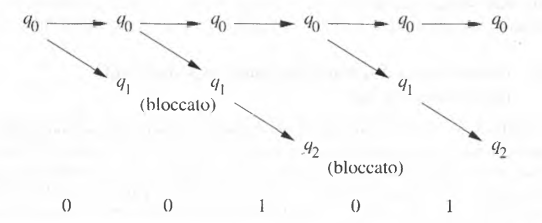
\includegraphics[scale=0.7]{img/nfa.png}
\end{center}
ovvero si parte dallo stato inziale, quando viene letto 0 si passa a $q_0$ e $q_1$, poi viene letto il secondo 0 quindi $q_0$ va nuovamente verso $q_0$ e $q_1$ mentre il primo $q_1$ muore non avendo transizioni su 0. Arriva poi l'1 quindi $q_0$ va solon verso $q_0$ e $q_1$ verso $q_2$ e sarebbe accettante ma l'input non è finito. Ora arriva 0 e $q_2$ si blocca mentre $q_0$ va sia in $q_0$ che in $q_1$. Arriva infine un 1 che manda $q_0$ in $q_0$ e $q_1$ in $q_2$ che è accettante e non avendo altri input si è dimostrata l'appartenenza della stringa al linguaggio
\end{esempio}
definisco quindi un NFA come una quintupla:
$$A=(Q,\Sigma,\delta,q_0,F)$$
con, a differenza dei DFA:
$$\delta:Q\times F\to 2^Q$$
Possiamo ora definire \^{$\delta$}, delta cappuccio che prende in ingresso uno stato e l'intera stringa $w$. Definisco ricorsivamente:
\begin{itemize}
\item \textbf{caso base:} se $|w|=0$ ovvero se $W=\varepsilon$ si ha:
$$\hat{\delta}(q,\varepsilon)=\{q\}$$
\item \textbf{caso passo:} se $|w|>0$, allora $W=xa$, $a\in\Sigma$ e $x\in\Sigma^*$. Posto $\hat{\delta}(q,x)=\{p_1,...,p_k\}$ si ha:
$$\hat{\delta}(q,w)=\\cup \delta(p_i,a)$$
\end{itemize}
%aggiungere esempio
Per il lingauggio $L$ accettato dall'automa si ha:
$$L(A)=\{w\in \Sigma^*|\, \hat{\delta}(q_0,q)\cap F\neq \emptyset\}$$
\begin{esempio}
Automa per $L=\{x010y|\,x,y\in\{0,1\}^*\}$ ovvero tutte le stringhe con dentro la sequenza $010$:
\begin{center}
\begin{tikzpicture}[shorten >=1pt,node distance=2cm,on grid,auto] 
\node[state, initial] (q_0) {$q_{0}$};
	\node[state] (q_1) [right=of q_0] {$q_{1}$};
	\node[state] (q_2) [right=of q_1] {$q_{2}$};
	\node[state, accepting] (q_3) [right=of q_2] {$q_{3}$};
	\path[->]
	(q_0) edge  node {0} (q_1)
	      edge [loop above] node {0,1} ()
	(q_1) edge  node {1} (q_2)
	(q_2) edge  node {0} (q_3)
	(q_3)     edge [loop above] node {0,1} ();
\end{tikzpicture}
\end{center}
\end{esempio}
Troviamo ora un algoritmo che trasformi un NFA in un DFA.\\
Dall'ultimo esempio ricavo:
\begin{center}
\begin{tabular}{c|c|c}
& 0 & 1\\
\hline
$\emptyset$ & $\emptyset$ & $\emptyset$ \\
\hline
$\to \,\{q_0\}$ & $\{q_0,q_1\}$ & $\{q_0\}$\\
\hline
$\,\{q_1\}$ & $\emptyset$ & $\{q_2\}$\\
\hline
$*\,\{q_2\}$ & $\emptyset$ & $\emptyset$\\
\hline
$\{q_0,q_1\}$ & $\{q_0,q_1\}$ & $\{q_0,q_2\}$\\
\hline
$*\,\{q_0,q_2\}$ & $\{q_0,q_1\}$ & $\{q_0\}$\\
\hline
$*\,\{q_1, q_2\}$ & $\emptyset$ & $\{q_2\}$\\
\hline
$*\,\{q_0,q_1,q_2\}$ & $\{q_0,q_1\}$ & $\{q_0,q_2\}$
\end{tabular}
\end{center}
ovvero:
\begin{center}
\begin{tikzpicture}[shorten >=1pt,node distance=4cm,on grid,auto] 
\node[state, initial] (q_0) {$\{q_{0}\}$};
	\node[state] (q_1) [right=of q_0] {$\{q_{0}, q_1\}$};
	\node[state] (q_2) [right=of q_1] {$\{q_0,q_{2}\}$};
	\path[->]
	(q_0) edge  node {0} (q_1)
	      edge [loop above] node {1} ()
	(q_1) edge  node {1} (q_2)
	      edge [loop above] node {0} ()
	(q_2) edge [bend left =25]  node {0} (q_1)
	      edge [bend left =45] node  {1} (q_0);
\end{tikzpicture}
\end{center}
che è il DFA che si era anche prima ottenuto. Si hanno però dei sottoinsiemi mai raggiungibili. Si ha quindi:
\begin{center}
\begin{tabular}{c|c|c}
& 0 & 1\\
\hline
$\to\,\{q_0\}$ & $\{q_0,q_1\}$ & $\{q_0\}$ \\
\hline
$\{q_0,q_1\}$ & $\{q_0,q_1\}$ & $\{q_0,q_2\}$\\
\hline
$\,\{q_0, q_2\}$ & $\{q_0,q_1\}$ & $\{q_0\}$
\end{tabular}
\end{center}
e definendo $\{q_0\}=a, \, \{q_0,q_1\}=b\,\,\, e\,\,\, \{q_0,q_2\}=c$ si avrà:
\begin{center}
\begin{tikzpicture}[shorten >=1pt,node distance=2cm,on grid,auto] 
	\node[state, initial] (q_0) {$a$};
	\node[state] (q_1) [right=of q_0] {$b$};
	\node[state, accepting] (q_2) [right=of q_1] {$c$};
	\path[->]
	(q_0) edge  node {0} (q_1)
	      edge [loop above] node {1} ()
	(q_1) edge  node {1} (q_2)
	      edge [loop above] node {0} ()
	(q_2) edge  [bend left =25] node {0} (q_1)
	      edge [bend left = 50] node {1} (q_0);
\end{tikzpicture}
\end{center}
Definiamo questo algoritmo che avrà:
\begin{itemize}
\item come input un NFA $N=(Q_n,\Sigma,\delta_N,q_0,F_N)$
\item come output un DFA $D=(Q_D,\Sigma,\delta_D,\{q_0\},F_D)$ tale che $L(D)=L(N)$
\end{itemize}
con:
\begin{itemize}
\item $Q_D=2^{Q_N}$ (quindi se $Q_N=n$ si ha $|Q_D|=2^n$)
\item $F_D=\{S\subseteq Q_n|\, S\cap F_N\neq \emptyset\}$
\item $\forall S\subseteq Q_N$ e $ \forall a \in\Sigma$:
$$\delta_D(S,a)=\cup \delta_n(p,a)$$
per esempio:
$$\delta_D(\{q_0,q_1,q_2\},0)=\delta_N(q_0,0)\cup \delta_N(q_1,0) \cup\delta_N(q_2,0) $$ 
\end{itemize}
Si definisce l'$\varepsilon-NFA$, l'automa astati finiti non deterministici con $\varepsilon$ transizioni. Con la transizione $\varepsilon$ posso saltare i nodi, ovvero avanza senza aggiungere caratteri
\begin{esempio}
Si ha $ER=a^*b^*c^*$, che genera:
$$L=\{a^nb^mc^k|\,n,m,k\geq 0\}$$
si ha:
\begin{center}
\begin{tikzpicture}[shorten >=1pt,node distance=2cm,on grid,auto] 
	\node[state, initial] (q_0) {$q_0$};
	\node[state] (q_1) [right=of q_0] {$q_1$};
	\node[state, accepting] (q_2) [right=of q_1] {$q_2$};
	\path[->]
	(q_0) edge  node {$\varepsilon$} (q_1)
	      edge [loop above] node {a} ()
	(q_1) edge  node {$\varepsilon$} (q_2)
	      edge [loop above] node {b} ()
	(q_2) edge  [loop above] node {c} ();
\end{tikzpicture}
\end{center}
ovvero con $\varepsilon$ posso per esempio generare quante $a$ voglio da $q_0$ e passare a $q_2$, uscendo senza generare altro
\end{esempio}
Si definisce la funzione $E\,CLOSE:Q\to 2^Q$, con $E\,CLOSE(q)$ insieme degli stati raggiungibili da $q$ tramite $\varepsilon-mosse$. Nell'esempio precedente si avrebbe:
$$E\,CLOSE(q_0)=\{q_0,q_1,q_2\}$$
$$E\,CLOSE(q_1)=\{q_1,q_2\}$$
$$E\,CLOSE(q_2)=\{q_2\}$$
si ha inoltre che:
\begin{itemize}
\item $E\,CLOSE 2^Q\to 2^Q\,\,\, P\subseteq Q$
\item $E\,CLOSE(P)=\cup E\,CLOSE(p)$
\item $E\,CLOSE(\emptyset)=\emptyset$
\end{itemize}
mettendo in tabella l'esempio precedente si ha:
\begin{center}
\begin{tabular}{c|c|c|c}
& a & b & c\\
\hline
$*\to\,\{q_0,q_1,q_2\}$ & $\{q_0,q_1,q_2\}$ & $\{q_1,q_2\}$ & $\{q_2\}$\\
\hline
$*\{q_1,q_2\}$ & $\emptyset$ & $\{q_1,q_2\}$ & $\{q_2\}$\\
\hline
$*\{q_2\}$ & $\emptyset$ & $\emptyset$ & $\{q_2\}$\\
\hline
$\emptyset$ & $\emptyset$ & $\emptyset$ & $\emptyset$ 
\end{tabular}
\end{center}
riscrivendo:
\begin{itemize}
\item $a=\{q_0,q_1,q_2\}$
\item $b=\{q_1,q_2\}$
\item $c=\{q_2\}$
\item $d=\emptyset$
\end{itemize}
ovvero:
$$\delta_D(\{q_0,q_1,q_2\},a)=E\,CLOSE(\delta_N(q_0,a)\cup \delta_N(q_1,a)\cup \delta_N(q_2,a))$$
$$=E\,CLOSE(\{q_0\} \cup \emptyset\cup \emptyset)=E\,CLOSE(\{q_0\})$$
$$=E\,CLOSE	(q_0)=\{q_0,q_1,q_2\}$$
e
$$\delta_D(\{q_0,q_1,q_2\},B)=E\,CLOSE(\delta_N(q_0,b)\cup \delta_N(q_1,b)\cup \delta_N(q_2,b))$$
$$=E\,CLOSE(\emptyset \cup \{q_1\}\cup \emptyset)=E\,CLOSE(\{q_1\})$$
$$=E\,CLOSE	(q_1)=\{q_1,q_2\}$$
e
$$\delta_D(\{q_0,q_1,q_2\},c)=E\,CLOSE(\delta_N(q_0,c)\cup \delta_N(q_1,c)\cup \delta_N(q_2,c))$$
$$=E\,CLOSE(\emptyset \cup \emptyset\cup \{q_2\})=E\,CLOSE(\{q_1\})$$
$$=E\,CLOSE	(q_2)=\{q_2\}$$
\newpage
si ottiene quindi il seguente NFA:
\begin{center}
\begin{tikzpicture}[shorten >=1pt,node distance=3cm,on grid,auto] 
	\node[state, initial, accepting] (q_0) {$A$};
	\node[state, accepting] (q_1) [right=of q_0] {$B$};
	\node[state, accepting] (q_2) [below=of q_0] {$C$};
	\node[state] (q_3) [right=of q_2] {$D$};
	\path[->]
	(q_0) edge  node {b} (q_1)
	      edge  node {c} (q_2)
	      edge [loop above] node {a} ()
	(q_1) edge  node {c} (q_2)
	      edge  node {a} (q_3)
	      edge [loop above] node {b} ()
	(q_2) edge  node {a,b} (q_3)
	      edge [loop below] node {c} ()
	(q_3) edge [loop below] node {a,b,c} ();
\end{tikzpicture}
\end{center}
che diventa il seguente DFA:
\begin{center}
\begin{tikzpicture}[shorten >=1pt,node distance=3cm,on grid,auto] 
	\node[state, initial, accepting] (q_0) {$\{q_0,q_1,q_2\}$};
	\node[state, accepting] (q_1) [right=of q_0] {$\{q_1,q_2\}$};
	\node[state, accepting] (q_2) [below=of q_0] {$\{q_2\}$};
	\node[state] (q_3) [right=of q_2] {$q_E$};
	\path[->]
	(q_0) edge  node {b} (q_1)
	      edge  node {c} (q_2)
	      edge [loop above] node {a} ()
	(q_1) edge  node {c} (q_2)
	      edge  node {a} (q_3)
	      edge [loop above] node {b} ()
	(q_2) edge  node {a,b} (q_3)
	      edge [loop below] node {c} ();
\end{tikzpicture}
\end{center}
\newpage
\subsubsection{esercizi}
\begin{esempio}
automa DFA per $w=x010y,\,x,y\in\{0,1\}^*$ :\\
la stringa più corta è 010
\begin{center}
\begin{tikzpicture}[shorten >=1pt,node distance=2cm,on grid,auto] 
\node[state, initial] (q_0) {$q_{0}$};
	\node[state] (q_1) [right=of q_0] {$q_{1}$};
	\node[state] (q_2) [right=of q_1] {$q_{2}$};
	\node[state, accepting] (q_3) [right=of q_2] {$q_{3}$};
	\path[->]
	(q_0) edge  node {0} (q_1)
	      edge [loop above] node {1} ()
	(q_1) edge  node {1} (q_2)
	      edge [loop above] node {0} ()
	(q_2) edge  node {0} (q_3)
	      edge  [bend left = 45] node {1}(q_0)
	(q_3) edge [loop above] node {0,1} ();
\end{tikzpicture}
\end{center}
\end{esempio}
\begin{esempio}
automa DFA per $a^{2k+1}b^{2h},\, h,k\geq 0$ :\\
concatenazione di a dispari e b pari:
\begin{center}
\begin{tikzpicture}[shorten >=1pt,node distance=2cm,on grid,auto] 
	\node[state, initial] (q_0) {$q_{0}$};
	\node[state, accepting] (q_1) [right=of q_0] {$q_{1}$};
	\node[state] (q_3) [right=of q_1] {$q_{3}$};
	\node[state] (q_2) [below= of q_1] {$q_{2}$};
	\node[state, accepting] (q_4) [right = of q_2] {$q_4$};
	\node[state] (q_5) [right=of q_4] {$q_E$};
	\path[->]
	(q_0) edge  node [bend left = 25] {a} (q_1)
	(q_1) edge [bend left = 25] node {a} (q_2)
	      edge node [bend left= 25] {b} (q_3)
	(q_2) edge [bend left = 25] node [left] {a} (q_1)
	(q_3) edge [bend right = 25] node [left] {b} (q_4)
	(q_4) edge [bend right = 25] node [right] {b} (q_3)
	(q_2) edge  [bend right = 55] node [below] {b} (q_5)
	(q_3) edge  [bend left = 25] node {a} (q_5)
	(q_4) edge  [bend right = 25] node [below] {a} (q_5)
	(q_5) edge [loop right] node {a,b} ();
\end{tikzpicture}
\end{center}
\end{esempio}
\begin{esempio}
cerco DFA per stringhe inizianti con a e finenti con b, con occorrenze di b singole o a coppie, nessuna regola per c.\\
per esempio $abbcb$ è nel linguaggio
\begin{center}
\begin{tikzpicture}[shorten >=1pt,node distance=2cm,on grid,auto] 
	\node[state, initial] (q_0) {$q_{0}$};
	\node[state] (q_1) [right=of q_0] {$q_{1}$};
	\node[state, accepting] (q_2) [right=of q_1] {$q_{2}$};
	\node[state, accepting] (q_3) [right= of q_3] {$q_{3}$};
	\node[state] (q_5) [below=of q_0] {$q_E$};
	\path[->]
	(q_0) edge  node [bend left = 25] {a} (q_1)
		  edge  node [bend left = 25] {b,c} (q_5)
	(q_1) edge  node {b} (q_2)
	      edge [loop] node {a,c} ()
	(q_2) edge [bend left = 25] node {a,c} (q_1)
	      edge  node  {b} (q_3)
	(q_3) edge [bend left = 65] node [below] {b} (q_5)
	      edge [bend left = 55] node {a,c} (q_1)
	(q_5) edge [loop left] node {a,b,c} ();
\end{tikzpicture}
\end{center}
\end{esempio}
\newpage
\begin{esempio}
cerco DFA per  stringhe di bit non contegano 000
\begin{center}
\begin{tikzpicture}[shorten >=1pt,node distance=2cm,on grid,auto] 
    \node[state, initial, accepting] (q_0) {$q_0$};
    \node[state, accepting] (q_1) [right=of q_0]{$q_1$};
    \node[state, accepting] (q_2) [right=of q_1]{$q_2$};
    \node[state] (q_e) [right=of q_2]{$q_E$};
    \path[->]
    (q_0) edge  [bend left=25] node {0} (q_1)
          edge [loop] node {1} ()
    (q_1) edge node {0} (q_2)
          edge [bend left=25] node {1} (q_0)
    (q_2) edge node {0} (q_e)
          edge  [bend left=55] node{1} (q_0)
    (q_e) edge [loop ] node {0,1} ();
\end{tikzpicture}
\end{center}
\end{esempio}
\begin{esempio}
cerco DFA per  stringhe di bit non contegano 000 almeno una volta
\begin{center}
\begin{tikzpicture}[shorten >=1pt,node distance=2cm,on grid,auto] 
    \node[state, initial] (q_0) {$q_0$};
    \node[state] (q_1) [right=of q_0]{$q_1$};
    \node[state] (q_2) [right=of q_1]{$q_2$};
    \node[state, accepting] (q_e) [right=of q_2]{$q_E$};
    \path[->]
    (q_0) edge  [bend left=25] node {0} (q_1)
          edge [loop] node {1} ()
    (q_1) edge node {0} (q_2)
          edge [bend left=25] node {1} (q_0)
    (q_2) edge node {0} (q_e)
          edge  [bend left=55] node{1} (q_0)
    (q_e) edge [loop ] node {0,1} ();
\end{tikzpicture}
\end{center}
\end{esempio}
\begin{esempio}
cerco DFA per  stringhe di bit che contengono 000 solo una volta
\begin{center}
\begin{tikzpicture}[shorten >=1pt,node distance=2cm,on grid,auto] 
    \node[state, initial] (q_0) {$q_0$};
    \node[state] (q_1) [right=of q_0]{$q_1$};
    \node[state] (q_2) [right=of q_1]{$q_2$};
    \node[state, accepting] (q_3) [right=of q_2]{$q_3$};
    \node[state,accepting] (q_4) [below=of q_3] {$q_3$};
    \node[state] (q_5) [below=of q_4]{$q_5$};
    \node[state] (q_6) [below=of q_5]{$q_6$};
    \node[state] (q_e) [right=of q_3]{$q_E$};
    \path[->]
    (q_0) edge  [bend left=25] node {0} (q_1)
          edge [loop] node {1} ()
    (q_1) edge node {0} (q_2)
          edge [bend left=25] node {1} (q_0)
    (q_2) edge node {0} (q_3)
          edge  [bend left=45] node{1} (q_0)
    (q_3) edge node {0} (q_e)
          edge node {1} (q_4)
    (q_4) edge [bend left=25] node {0} (q_5)
    	  edge [loop right] node {1} ()
    (q_5) edge [bend left=25] node {1} (q_4)
          edge node {0} (q_6)
    (q_6) edge [bend right=25] node {0} (q_e)
          edge [bend left=55] node {0} (q_4)
    (q_e) edge [loop ] node {0,1} ();
\end{tikzpicture}
\end{center}
\end{esempio}
\newpage
\begin{esempio}
Trasformare il seguente NFA in un DFA:
\begin{center}
\begin{tikzpicture}[shorten >=1pt,node distance=3cm,on grid,auto] 
	\node[state, initial, accepting] (q_0) {$q_0$};
	\node[state, accepting] (q_1) [above right=of q_0] {$q_1$};
	\node[state] (q_2) [below right =of q_0] {$q_2$};
	\node[state] (q_3) [below right=of q_1] {$q_3$};
	\path[->]
	(q_0) edge  [bend left=25] node {a} (q_1)
	      edge  [bend right=25] node [below] {b} (q_2)
	(q_1) edge  [bend left=25] node {a} (q_2)
	      edge [loop ] node {a} ()
	(q_2) edge  [bend left=25] node {b} (q_1)
	      edge  [bend right=15] node [below] {b} (q_3)
	(q_3) edge   node [above] {a} (q_1)
	      edge  [bend right=15] node [above] {a} (q_2);
\end{tikzpicture}
\end{center}
abbiamo quindi:
$$\delta_D(\{q_0\},a)=\delta_N(q_0,a)=\{q_1,q_2\}$$
$$\delta_D(\{q_0\},b)=\delta_N(q_1,b)=\emptyset$$
$$\delta_D(\{q_1,q_2\},a)=\delta_N(q_1,a)\cup \delta_N(q_2,a)=\{q_1,q_2\}cup \emptyset=\{q_1,q_2\}$$
$$\delta_D(\{q_1,q_2\},b)=\delta_N(q_1,b)\cup \delta_N(q_2,b)=\emptyset\cup \{q_1,q_3\}=\{q_1,q_3\}$$
$$...$$
ottengo quindi:
\begin{center}
\begin{tabular}{c|c|c}
DFA & a & b \\
\hline
$*\to\,\{q_0\}$ & $\{q_1,q_2\}$ & $\emptyset$ \\
\hline
$*\{q_1,q_2\}$ & $\{q_1,q_2\}$ & $\{q_1,q_3\}$ \\
\hline
$\emptyset$ & $\emptyset$ & $\emptyset$ \\
\hline
$*\{q_1,q_3\}$ & $\{q_1,q_2\}$ & $\emptyset$ 
\end{tabular}
\end{center}
Posso ora rinominare:
\begin{itemize}
\item $A=\{q_0\}$
\item $B=\{q_1,q_2\}$
\item $C=\emptyset$
\item $D=\{q_1,q_3\}$
\end{itemize}
\newpage
ottengo quindi il seguente DFA:
\begin{center}
\begin{tikzpicture}[shorten >=1pt,node distance=3cm,on grid,auto] 
	\node[state, initial, accepting] (q_0) {$A$};
	\node[state, accepting] (q_1) [right=of q_0] {$B$};
	\node[state] (q_2) [below=of q_0] {$C$};
	\node[state,accepting] (q_3) [right=of q_2] {$D$};
	\path[->]
	(q_0) edge  node {a} (q_1)
	      edge  node {b} (q_2)
	(q_1) edge  [bend left=25] node {b} (q_3)
	      edge  [loop] node {a} ()
	(q_2) edge  [loop below] node {a,b} ()
	(q_3) edge  [bend left=25] node {a} (q_1)
	      edge  node  {a} (q_2);
\end{tikzpicture}
\end{center}
\end{esempio}
\begin{esempio}
Trasformare il seguente $\varepsilon$-NFA in un DFA:
\begin{center}
\begin{tikzpicture}[shorten >=1pt,node distance=3cm,on grid,auto] 
	\node[state, initial] (q_0) {$p$};
	\node[state] (q_1) [right=of q_0] {$q$};
	\node[state, accepting] (q_2) [below right =of q_0] {$r$};
	\path[->]
	(q_0) edge  [bend left=25] node [left] {c} (q_2)
	      edge  [bend right=25] node {b} (q_1)
	      edge [loop ] node {a} ()
	(q_1) edge  [bend right=25] node {$\varepsilon$} (q_0)
	      edge  [bend right=25] node [left] {b} (q_2)
	      edge  [loop ] node {a} ()
	(q_2) edge  [bend left=25] node {c} (q_0)
	      edge  [bend right=25] node [right] {$\varepsilon$} (q_1)
	      edge  [loop below] node {a} ();
\end{tikzpicture}
\end{center}
vediamo le ECLOSE:
$$ECLOSE(p)=\{p\}$$
$$ECLOSE(q)=\{p,q\}$$
$$ECLOSE(r)=\{p,q,r\}$$
si ottiene quindi:
\begin{center}
\begin{tabular}{c|c|c|c}
 & a & b & c\\
\hline
$to\,\{p\}$ & $\{p\}$ & $\{p,q\}$ & $\{p,q,r\}$\\
\hline
$\{p,q\}$ & $\{p,q\}$ & $\{p,q,r\}$ & $\{p,q,r\}$\\
\hline
$*\{p,q,r\}$ & $\{p,q,r\}$ & $\{p,q,r\}$ & $\{p,q,r\}$
\end{tabular}
\end{center}
infatti, per esempio:
$$\delta_D(\{p\}, a)= ECLOSE (\delta_(p,a))=ECLOSE (\{p\})=ECLOSE (p)=\{p\}$$
$$\delta_D(\{p,q\}, a)= ECLOSE (\delta_N(p,a)\cup \delta_N(q,a))=$$
$$ECLOSE (\{p\}\cup \{q\})=ECLOSE(P)\cup ECLOSE(q)=\{p\}\cup\{p,q\}=\{p,q\}$$
$$...$$
si hanno quindi le seguenti rinominazioni:
\begin{itemize}
\item $A=\{p\}$
\item $b=\{p,q\}$
\item $C=\{p,q,r\}$
\end{itemize}
ovvero:
\begin{center}
\begin{tikzpicture}[shorten >=1pt,node distance=3cm,on grid,auto] 
	\node[state, initial] (q_0) {$A$};
	\node[state] (q_1) [right=of q_0] {$B$};
	\node[state, accepting] (q_2) [below=of q_0] {$C$};
	\path[->]
	(q_0) edge  node {b} (q_1)
	      edge  node {c} (q_2)
	      edge  [loop] node {a} ()
	(q_1) edge  node {b,c} (q_2)
	      edge  [loop] node {a} ()
	(q_2) edge  [loop below] node {a,b,c} ();
\end{tikzpicture}
\end{center}
\end{esempio}
\newpage
torniamo a dare bene qualche definizione per \^{$\delta$} in un DFA:
\begin{center}
\^{$\delta$}$:Q\times \Sigma^* \to Q$
\end{center}
con: $q\in Q,\,\,\, w\in \Sigma^*\,\,\,e\,\,\,$\^{$\delta$}$(p,w)=q$
\begin{itemize}
\item 
\textbf{caso base:} $w=\varepsilon\to |w|=0\to$\^{$\delta$}$(q,\varepsilon)=q$
\\
\textbf{caso passo:} $|w|\neq0\to w=ax$ con $a\in \Sigma,x\in \Sigma^*$:
\^{$\delta$}$(q,w)=$\^{$\delta$}$(q,ax)=$\^{$\delta$} $(\delta(q,a),x)$
\item 
\textbf{caso base:} $w=\varepsilon\to |w|=0\to \delta(q,w)=\delta(q,\varepsilon)=q$
\\
\textbf{caso passo:} $|w|\neq0\to w=xa$ con $a\in \Sigma,x\in \Sigma^*$:
\^{$\delta$}$(q,w)=$\^{$\delta$}$(q,xa)=$\^{$\delta$} $(\delta(q,x),a)$
\end{itemize}
in un NFA si ha:
\begin{itemize}
\item \textbf{caso base:}  \^{$\delta$}$(q,\varepsilon=\{q\},\,\,\forall q\in Q$
\item \textbf{caso passo:} posto $w=ax$ e \^{$\delta$}$(q,a)=\{p_1,...,p_n\`$ allora \^{$\delta$}$(q,w)=\cup$\^{$\delta$}$(p_i, x)0\{r_1,...,r_n\}$.\\
 \^{$\delta$}$(q,a)=p$\\
  \^{$\delta$}$(q,w)=$ \^{$\delta$}$(q,xa)=$ \^{$\delta$}$(p,x)=r$
\end{itemize}
oppure:
\begin{itemize}
\item \textbf{caso base:}  \^{$\delta$}$(q,\varepsilon)=\{q\},\,\forall q\in Q$
\item \textbf{caso passo:} posto $w=xa$ si ha  \^{$\delta$}$(q,q)=$ \^{$\delta$}$(q,xa)=\cup \delta(p,a)$ con  \^{$\delta$}$(q,x)=\{p_1,...,p_n\}$
\end{itemize}
Se ho un NFA $N=(Q_N, \Sigma, \delta_N, q_{0_N}, F_N)$ con $\delta_N: Q\times\Sigma^*\to 2^{Q_N}$ che accetta un lingiaggio $L$ posso ottenere un DFA $D=(Q_D, \Sigma, \delta_D, q_{0_D}, F_D)$ equivalente con $Q_D=2^{Q_N}$  e $q_{0_D}=\{q_{0_N}\}$ che accetta L.\\
$\forall S\subseteq Q_N$ e $\forall a\in \Sigma$ si ha:
$$F_D=\{S\subseteq Q_N\,|\, S\cap F_n\neq \emptyset\}$$
con $\delta_D(S,a)=\cup \delta_N(p,a)$
 Si ha che:
$$|Q_D|=|2^{Q_N}|=2^{|Q_N|}$$
partiamo con un esempio:
\begin{center}
\begin{tikzpicture}[shorten >=1pt,node distance=2cm,on grid,auto] 
gin{tikzpicture}[shorten >=1pt,node distance=2cm,on grid,auto] 
   \node[state,initial] (q_0)   {$q_0$}; 
   \node[state] (q_1) [right=of q_0] {$q_1$}; 
   \node[state] (q_2) [right=of q_1] {$...$}; 
   \node[state] (q_3) [right=of q_2] {$q_{n-1}$}; 
   \node[state, accepting] (q_4) [right=of q_3] {$q_n$}; 
   \path[->] 
   (q_0) edge  node {1} (q_1)
         edge [loop above] node {0,1} ()
   (q_1) edge  node {0,1} (q_2)
   (q_2) edge node {0,1} (q_3)
   (q_3) edge node {0,1} (q_4);
\end{tikzpicture}
\end{center}
che definisce un $L\subseteq\{0,1\}^*$ tale che $w\in L$ sse n-simo elemento della fine è 1. Si ha:
$$|Q_N|=n+1\to |Q_D|=2^n$$
Si ha che dato un $\varepsilon$-NFA $E=(Q_E, \Sigma, \delta_E, q_{0_E}, F_E)$ che riconosce $L$ in un NFA $N=(Q_N, \Sigma, \delta_N, q_{0_N}, F_N)$ equivalenti con $Q_N=2^{Q_E}$ stati in $Q_E$ $\varepsilon$-close: \textit{ECLOSE(S)=S} e $q_N=ECLOSE(q_E)$:
$$F_N\{S\in Q_F,\,\, S\subseteq Q_E | S\cap F_E\neq \emptyset\}$$
quindi:
$$\forall a\in \Sigma \mbox{ e } \forall S=\{p_1,...,p_k\}, \forall S\in Q_F \mbox{ e } Q_E$$
$$\delta_F(S,a) \mbox{ si ottiene }\cup \delta_E(p_i,a)=\{r_1,..., r_n\}$$
$$\delta_N(S,a)=ECLOSE(\{r_1, ..., r_n\})$$
\newpage
\subsection{Da espressioni regolari a automi E-NFA}
\begin{itemize}
\item \textbf{caso base}:
\begin{enumerate}
\item se $R=\varepsilon$ ovvero $L(R)=\{\varepsilon\}$ allora:
\begin{center}
\begin{tikzpicture}[shorten >=1pt,node distance=2cm,on grid,auto] 
   \node[state,initial] (q_0)   {$q_0$}; 
   \node[state, accepting] (q_1) [right=of q_0] {$q_1$}; 
   \path[->]
   (q_0) edge node {$\varepsilon$} (q_1);
\end{tikzpicture}
\end{center}
\item se $R=\emptyset$ ovvero $L(R)=\emptyset$ allora:
\begin{center}
\begin{tikzpicture}[shorten >=1pt,node distance=2cm,on grid,auto] 
   \node[state,initial] (q_0)   {$q_0$}; 
   \node[state, accepting] (q_1) [right=of q_0] {$q_1$}; ;
\end{tikzpicture}
\end{center}
\item se $R=a$ ovvero $L(R)=\{a\}$ allora:
\begin{center}
\begin{tikzpicture}[shorten >=1pt,node distance=2cm,on grid,auto] 
   \node[state,initial] (q_0)   {$q_0$}; 
   \node[state, accepting] (q_1) [right=of q_0] {$q_1$};
   \path[->]
   (q_0) edge node {a} (q_1);
\end{tikzpicture}
\end{center}
\end{enumerate}
\item \textbf{caso passo:}
\begin{enumerate}
\item se $R=S+T$ quindi $L(R)=L(S)+L(T)$ allora:
\begin{center}
\begin{tikzpicture}[shorten >=1pt,node distance=2cm,on grid,auto] 
   \node[state,initial] (q_0)   {$q_0$}; 
   \node[state] (q_1) [above right =of q_0] {$q_1$};
   \node[state] (q_2) [below right =of q_0] {$q_2$};
   \node[draw=none,fill=none] (Q_E) [right = of q_1] {$S$};
   \node[draw=none,fill=none] (Q_F) [right = of q_2] {$S$};
   \node[state] (q_3) [right=of Q_E] {$q_3$};
   \node[state] (q_4) [right=of Q_F] {$q_4$};
   \node[state, accepting] (q_5) [below right =of q_3] {$q_5$};
   \path[->]
   (q_0) edge node {$\varepsilon$} (q_1)
   (q_0) edge node {$\varepsilon$} (q_2)
   (q_3) edge node {$\varepsilon$} (q_5)
   (q_4) edge node {$\varepsilon$} (q_5);
\end{tikzpicture}
\end{center}
\item se $R=ST$ quindi $L(R)=L(S)L(T)$:
\begin{center}
\begin{tikzpicture}[shorten >=1pt,node distance=2cm,on grid,auto] 
   \node[state,initial] (q_0)   {$q_0$};
   \node[draw=none,fill=none] (Q_E) [right = of q_0] {$S$}; 
   \node[state] (q_1) [ right =of Q_E] {$q_1$};
   \node[state] (q_2) [right =of q_1] {$q_2$};
   \node[draw=none,fill=none] (Q_F) [right = of q_2] {$T$};
   \node[state] (q_3) [right=of Q_F] {$q_3$};
   \node[draw=none,fill=none] (Q_G) [right = of q_3] {};
   \path[->]
   (q_1) edge node {$\varepsilon$} (q_2)
   (q_3) edge node {} (Q_G);
\end{tikzpicture}
\end{center}
\item se $R=S^*$ quindi $L(R)=(L(S))^*$:
\begin{center}
\begin{tikzpicture}[shorten >=1pt,node distance=2cm,on grid,auto] 
   \node[state,initial] (q_0)   {$q_0$}; 
   \node[state] (q_1) [ right =of Q_E] {$q_1$};
   \node[draw=none,fill=none] (Q_F) [right = of q_1] {$S$};
   \node[state] (q_2) [right =of Q_F] {$q_2$};
   \node[state] (q_3) [right=of q_2] {$q_3$};
   \path[->]
   (q_0) edge node {$\varepsilon$} (q_1)
   (q_2) edge [bend right = 35]  node {$\varepsilon$} (q_1)
   (q_0) edge [bend right = 25] node  {$\varepsilon$} (q_3)
   (q_2) edge node {$\varepsilon$} (q_3);
\end{tikzpicture}
\end{center}
\end{enumerate}
\end{itemize}
\newpage
\begin{esempio}

\end{esempio}
\end{document}